\documentclass[
  aps,
  prb,
  reprint,
  amsmath,
  amssymb,
  superscriptaddress,
  longbibliography,
  nofootinbib,
  floatfix,
  showkeys
]{revtex4-2}

\usepackage[T1]{fontenc}
\usepackage{lmodern}
\usepackage{graphicx}
\usepackage{bm}
\usepackage{booktabs}
\usepackage{siunitx}
\usepackage{xcolor}
\usepackage{microtype}
\usepackage{hyperref}

\hypersetup{
  colorlinks=true,
  linkcolor=blue!50!black,
  citecolor=green!35!black,
  urlcolor=blue!60!black
}

\graphicspath{{figures/}}
\sisetup{separate-uncertainty=true}

\newcommand{\Heff}{H_{\mathrm{eff}}}
\newcommand{\Jeff}{J_{\mathrm{eff}}}
\newcommand{\ceff}{c_{\mathrm{eff}}}
\newcommand{\qpeak}{q_{\mathrm{peak}}}
\newcommand{\Szz}{S^{zz}(q,\omega)}
\newcommand{\avg}[1]{\left\langle #1\right\rangle}

\begin{document}

\title{Local multiplets, effective-chain dynamics, and momentum reconstruction in a spin-\texorpdfstring{$1/2$}{1/2} Heisenberg pentamer chain}

\author{Author Name}
\email{corresponding.author@example.edu}
\affiliation{Department and Institution, City, Postal Code, Country}

\date{\today}

\begin{abstract}
Clusterized quantum spin chains connect local few-spin multiplets to extended many-body excitations.
We investigate a spin-$1/2$ Heisenberg chain with a five-site unit cell using exact diagonalization, low-energy projection, finite-size density-matrix renormalization group calculations, entanglement diagnostics, correction-vector spectra, and real-time matrix-product-state dynamics.
For positive intra-cell and inter-cell couplings, the isolated pentamer retains an even-reflection-parity spin-$1/2$ ground-state doublet.
Projecting the inter-cell exchange onto this doublet gives an antiferromagnetic effective Heisenberg chain, and the leading correction to the projected energy is quadratic in the inter-cell coupling.
Matched-size entanglement estimates, small finite-size spin gaps, algebraic correlations, and a dominant response at $q=\pi$ are consistent with a $c=1$ effective-chain description at the tested positive-coupling points.
Reflection parity suppresses the lowest excited doublet at $q=\pi$, whereas spin-$3/2$ multiplets carry $84.1\%$--$97.6\%$ of the isolated-pentamer inelastic weight.
Correction-vector and time-evolution calculations connect these local selection rules to the collective spectrum.
In the negative-$\alpha$ region, 96 parameter--size records at 48 coupling points were evaluated, with 89 accepted and seven retained as bounded records.
A further 29 $L=60,80$ refinement cells passed the complete numerical and provenance chain.
The dominant finite-size momentum reconstructs from approximately $0.60\pi$ to $\pi$, but none of eight candidate intervals satisfies the predeclared momentum and finite-size-flow criteria simultaneously.
A final $k=8\rightarrow12$ Krylov-subspace control leaves $\qpeak/\pi=1$ unchanged at the most solver-sensitive $L=80$ point.
We therefore identify a robust finite-size momentum reconstruction, retain crossover as the working interpretation, and withhold a separate thermodynamic phase label.
\end{abstract}

\keywords{Heisenberg chain, pentamer, matrix-product states, dynamical structure factor, finite-size scaling}

\maketitle

\section{Introduction}
\label{sec:introduction}

Clusterized quantum magnets provide a direct route from the spectrum of a few-spin unit to the collective behavior of a quantum many-body system.
Their local multiplets can survive as low-energy degrees of freedom, become dispersive, or be removed from an experimental response by symmetry.
Clusterized chains therefore separate three questions that are often mixed together in a conventional phase diagram: which local state remains active, how neighboring units couple, and which resulting excitations are visible.

The recent spin-$1/2$ tetramer-chain study provides a useful reference because it treats magnetic order, entanglement structure, and excitation spectra within a common coupling diagram~\cite{li2026tetramer_verified}.
Replacing four spins by five is not, however, a minor geometric modification.
A unit cell with an odd number of half-integer spins retains a half-integer degree of freedom unless symmetry breaking or ground-state degeneracy intervenes.
Lieb--Schultz--Mattis-type results therefore constrain a unique symmetry-preserving gapped ground state under the relevant translation and spin-rotation assumptions~\cite{lieb1961,ogata2019}.
This constraint does not determine the phase diagram and does not by itself establish a globally gapless $c=1$ state.

Here we study a linear Heisenberg pentamer chain with two intra-cell exchanges, $J_1$ and $J_2$, and an inter-cell exchange $J_3$.
We set $J_1=1$ and define $\alpha=J_2/J_1$ and $\beta=J_3/J_1$.
The geometry differs from previously studied mixed-spin or differently connected pentamers, so their multiplet assignments cannot be transferred directly to the present model~\cite{haraldsen2011}.
Instead, we determine the complete isolated-cell spectrum, construct the low-energy projected chain, and test the resulting picture against static and dynamical many-body calculations.

Three results organize this work.
First, throughout the sampled positive-$\alpha$ region, the pentamer ground state is an even-parity spin-$1/2$ doublet and positive $\beta$ generates an antiferromagnetic effective chain.
Second, reflection parity makes the lowest excited doublet essentially dark at $q=\pi$ and concentrates the local inelastic weight in spin-$3/2$ multiplets.
Third, negative $\alpha$ produces a reproducible finite-size reconstruction of the dominant momentum.
The last result is not promoted to a thermodynamic phase boundary because two independently declared diagnostics do not localize the same adjacent interval.

This distinction between a resolved microscopic mechanism and a bounded phase-diagram statement is central to our analysis.
Production records are accepted only after numerical, transfer, checksum, and independent-validator gates.
We retain the raw spectral ringing, distinguish the Krylov dimension $k$ from the matrix-product-state bond dimension $\chi$, and report initial-state differences as systematic sensitivity rather than statistical uncertainty.


\section{Model and numerical methods}
\label{sec:methods}

\subsection{Hamiltonian and isolated-cell projection}

The Hamiltonian is
\begin{align}
H={}&J_1\sum_n\left(\bm S_{n,2}\!\cdot\!\bm S_{n,3}
 +\bm S_{n,3}\!\cdot\!\bm S_{n,4}\right) \notag\\
&+J_2\sum_n\left(\bm S_{n,1}\!\cdot\!\bm S_{n,2}
 +\bm S_{n,4}\!\cdot\!\bm S_{n,5}\right) \notag\\
&+J_3\sum_n\bm S_{n,5}\!\cdot\!\bm S_{n+1,1}.
\label{eq:hamiltonian}
\end{align}
The isolated pentamer has a 32-dimensional Hilbert space.
We diagonalize it completely and resolve each degenerate energy subspace by total spin and reflection parity.
Spectral weights are evaluated with projectors onto complete multiplets, avoiding the arbitrary orientation of individual eigenvectors within a degenerate subspace.

If $P$ projects onto the ground-state doublet, the local spins satisfy
\begin{equation}
P\bm S_{n,a}P=c_a\bm T_n,
\label{eq:projection}
\end{equation}
where $\bm T_n$ is an effective spin-$1/2$ operator.
To leading order in the inter-cell coupling,
\begin{equation}
\Heff=NE_5+\Jeff\sum_n\bm T_n\cdot\bm T_{n+1}+O(\beta^2),
\qquad \Jeff=\beta c_1c_5.
\label{eq:effective}
\end{equation}
We test the projection using exact diagonalization of two coupled pentamers and finite-chain calculations with $N=8,12,16$ pentamers.

\begin{figure*}[t]
  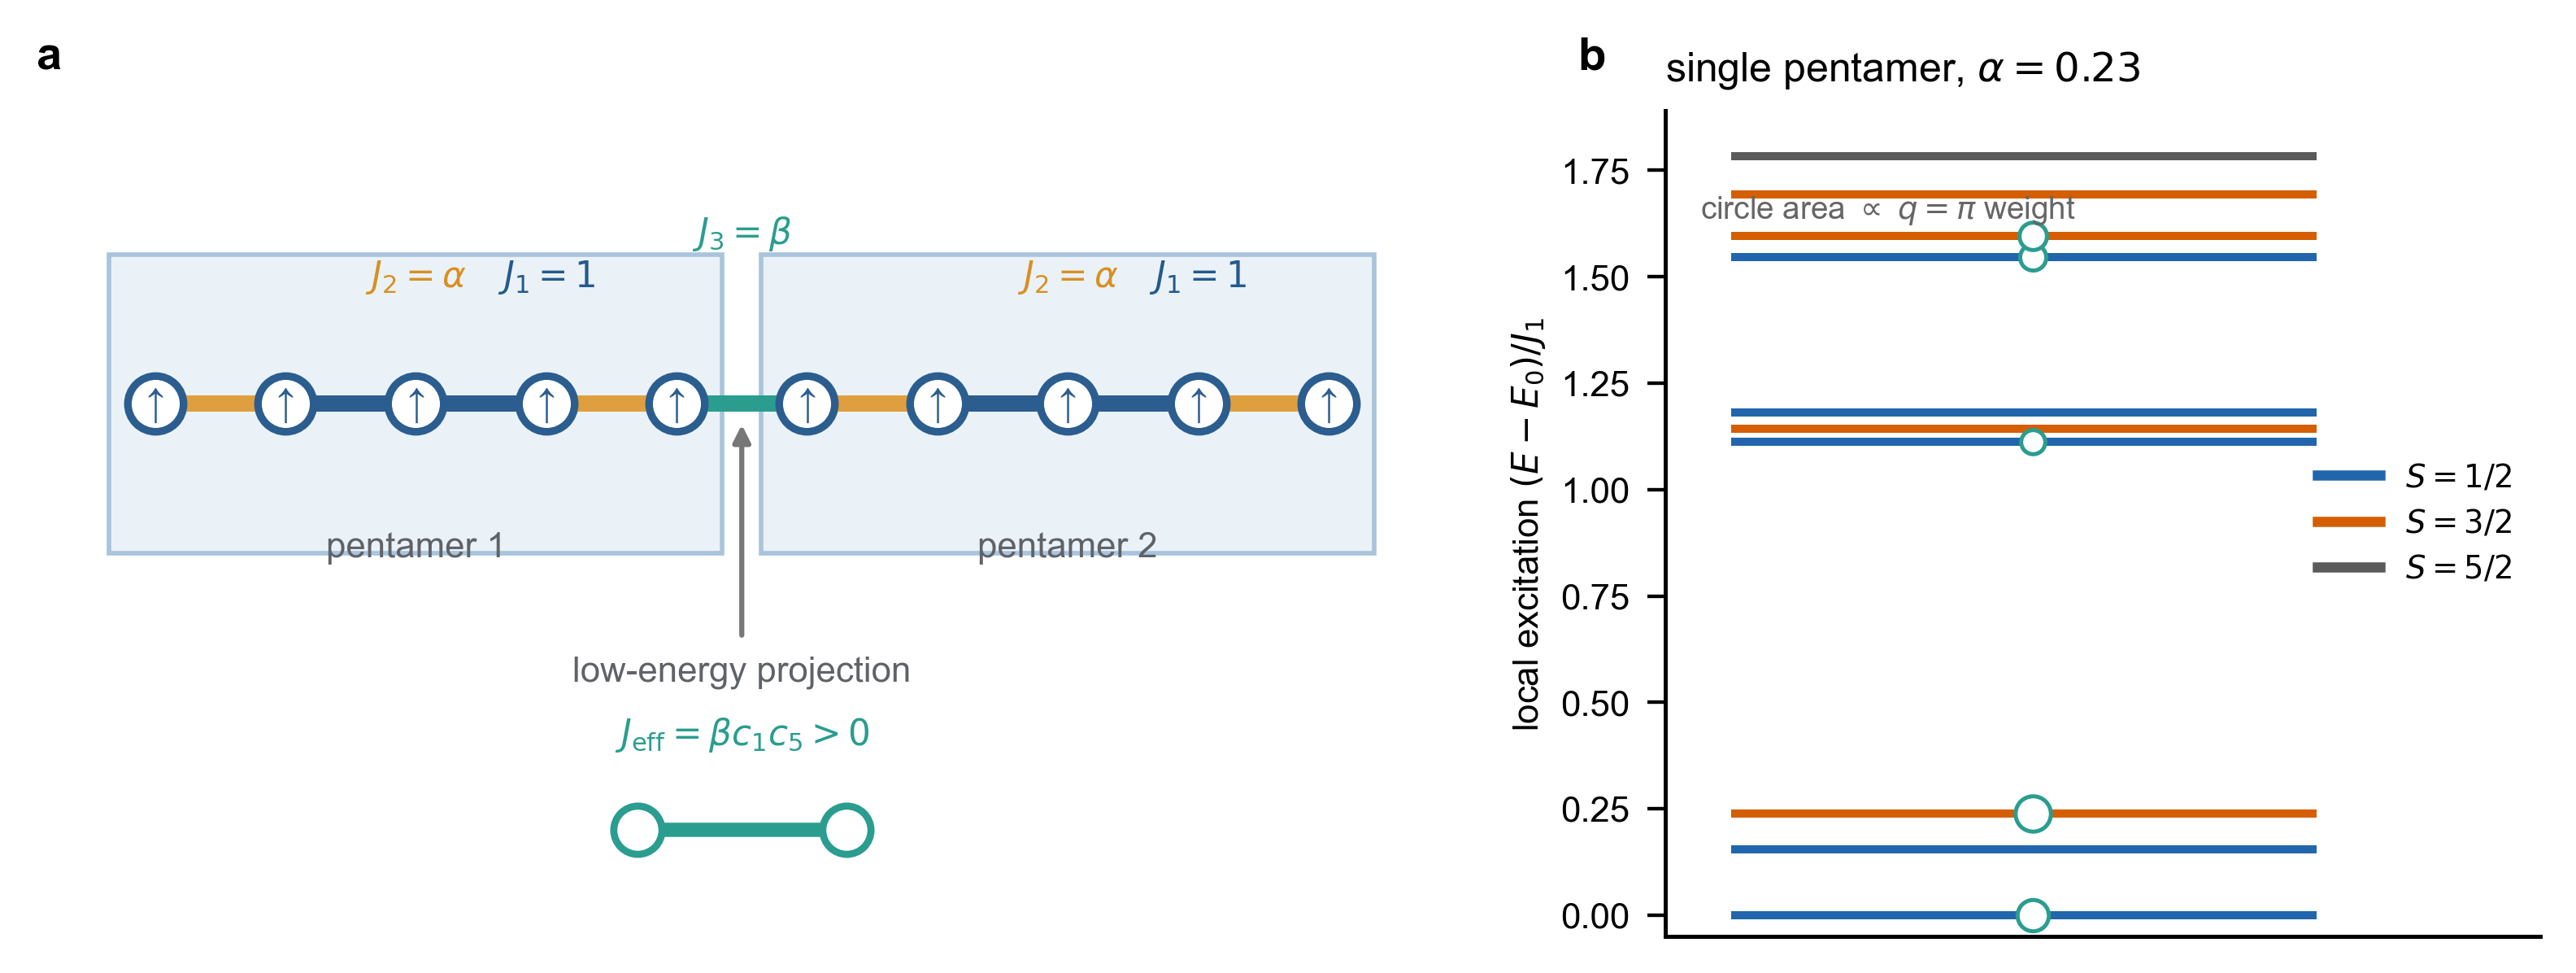
\includegraphics[width=\textwidth]{fig1_model_projection.png}
  \caption{Model and low-energy projection.
  The five-site unit cell defines the couplings $J_1$, $J_2$, and $J_3$.
  Isolated-pentamer multiplets are resolved by total spin and reflection parity, and the ground-state doublet is projected onto an effective spin-$1/2$ degree of freedom.}
  \label{fig:model}
\end{figure*}

\subsection{Static finite-chain calculations and acceptance gates}

Finite chains use open boundaries and $L=5N$ physical spins.
Ground states are obtained in fixed total-$S^z$ sectors with density-matrix renormalization group calculations in a matrix-product-state representation~\cite{white1992,schollwoeck2011}.
Sector-specific initial states are used rather than assuming that one initialization samples every low-energy solution.

The positive-region data set contains 105 accepted records at $L=40,60,80$.
For negative $\alpha$, the Practical V2 protocol uses the \texttt{center} and \texttt{ferro\_j2} product-state initializations in the $S^z=0$ sector and a fixed \texttt{center} initialization in the $S^z=1$ sector.
A new record is accepted only if
\begin{align}
\frac{\mathrm{Var}(H)}{L}&\leq5\times10^{-8}, \notag\\
\epsilon_{\mathrm{trunc}}&\leq10^{-9}, \notag\\
|S^z-S^z_{\mathrm{target}}|&\leq10^{-8},
\label{eq:gates}
\end{align}
and the sector gap is no smaller than $-10^{-8}$.
New Practical V2 calculations use at most 64 sweeps.
The two $S^z=0$ initial states test initialization sensitivity and are not independent statistical replicates.

Every accepted remote result is checked by parent and child manifests, transferred without overwriting earlier runs, checked again locally, and passed through an independent validator.
Records that fail a gate are retained as bounded or not evaluable and are excluded from accepted-only boundary inference.

\subsection{Entanglement, correlation, and momentum diagnostics}

For an open critical chain, the bond entropy is compared with
\begin{equation}
S(b)=a_g+\frac{\ceff}{6}
\ln\left[\frac{2L}{\pi}\sin\left(\frac{\pi b}{L}\right)\right].
\label{eq:entropy}
\end{equation}
The intercept $a_g$ depends on the bond class $g=b\bmod 5$ or $b\bmod 10$, while a common slope defines the descriptive coefficient $\ceff$.
Fits use central windows $fL\leq b\leq(1-f)L$ with $f=0.10$, 0.15, 0.20, and 0.25.
We call this quantity an effective entropy coefficient rather than a central charge unless size and solver controls justify the stronger interpretation~\cite{calabrese2004}.

The negative-$\alpha$ scan tracks the dominant structure-factor momentum $\qpeak$ and a dominant-ratio observable $R_L$.
A candidate boundary is retained only when an adjacent coupling interval shows both a momentum reconstruction and a consistent finite-size signature in $\Delta R=R_{80}-R_{60}$.

\subsection{Dynamical structure factor}

We compute the dynamical structure factor by two independent matrix-product-state routes.
Correction-vector DMRG gives a fixed-frequency spectrum at $q=\pi$~\cite{kuehner1999}.
Real-time evolution followed by Fourier transformation provides the full momentum dependence and an independent line-shape check~\cite{vidal2004,fishman2022}.
The correction-vector implementation reproduces the complete $L=10$ spectrum with relative $L_2$ error $8.52\times10^{-12}$.

The production full-momentum calculations use $L=40$, $t_{\max}=30$, 121 momentum points, 301 frequency points, and paired time steps $\Delta t=0.025$ and 0.0125.
The raw Fourier matrices, including negative ringing from the finite time window, are retained and tested rather than clipped.

\subsection{Krylov-subspace stability control}

The saved-state anomaly at $(\alpha,\beta)=(-0.10,0.25)$ was the point most sensitive to the local eigensolver configuration.
We therefore performed an $L=80$ control in which all physical and DMRG settings were fixed while the Krylov dimension increased from $k=8$ to 12.
Both $S^z=0$ initial states used 64 sweeps, configured maximum bond dimension 1200, cutoff $10^{-11}$, and the same 401-point momentum grid.
The symbol $k$ denotes the Krylov-subspace dimension and is distinct from the MPS bond dimension $\chi$.

The $k=12$ run passed the remote and local checksum chain and the Practical V2 validator.
Its variance per site was $1.86$--$1.87\times10^{-11}$, and the two sector gaps were $7.2772047002\times10^{-5}$ and $7.2772051798\times10^{-5}$.
Across 172 matched records, the $k=8\rightarrow12$ differences were bounded by $7.5211\times10^{-12}$ for the spin gap, $8.3994\times10^{-8}$ for the dominant ratio, and $5.7413\times10^{-8}$ for the entropy.
The value $\qpeak/\pi=1$ was unchanged.
The bond dimensions actually retained at this size were well below the configured cap and nearly insensitive to the solver change: the largest link dimension was 264--265 in the $S^z=0$ sector and 186--190 in $S^z=1$, against a configured maximum of 1200.

Two disclosures bound how these controls may be combined.
First, the $k=3\rightarrow8$ comparison is a solver-control audit, not a convergence proof, and the observed link dimensions are not a convergence statement: $k$ is the Krylov dimension, the retained bond dimension is $\chi$, and no $\chi$ series was performed.
Second, the historical negative-$\alpha$ records, including the $L=40$ and $L=60$ entries of the size comparison in Sec.~\ref{sec:results}, were produced with the earlier Krylov configuration; only the $L=80$ endpoint carries a $k=8$ control.
Records with different solver settings are therefore not combined into a finite-size scaling series, and no thermodynamic extrapolation is drawn from them.

\section{Results}
\label{sec:results}

\subsection{The odd pentamer retains a low-energy spin doublet}

At all 100 sampled points with $0<\alpha\leq1$, the isolated-pentamer ground state is an even-reflection-parity spin-$1/2$ doublet.
The lowest excited doublet is odd under reflection, whereas the lowest spin-$3/2$ multiplet is even.
The five-spin unit therefore retains an active half-integer degree of freedom instead of forming a fully quenched singlet cluster.

At $\alpha=0.14$, 0.23, and 0.33, the projected coupling satisfies $\Jeff/\beta=0.4396$, 0.4318, and 0.4189, respectively.
Positive $\beta$ therefore generates an antiferromagnetic effective spin-$1/2$ chain.
The residual between projected and exact ground-state energies scales with powers 1.9689--1.9915 for two coupled pentamers and 1.9483--1.9495 for complete chains with $N=8,12,16$.
The leading correction is consistent with the $O(\beta^2)$ term in Eq.~\eqref{eq:effective}.

\begin{figure*}[t]
  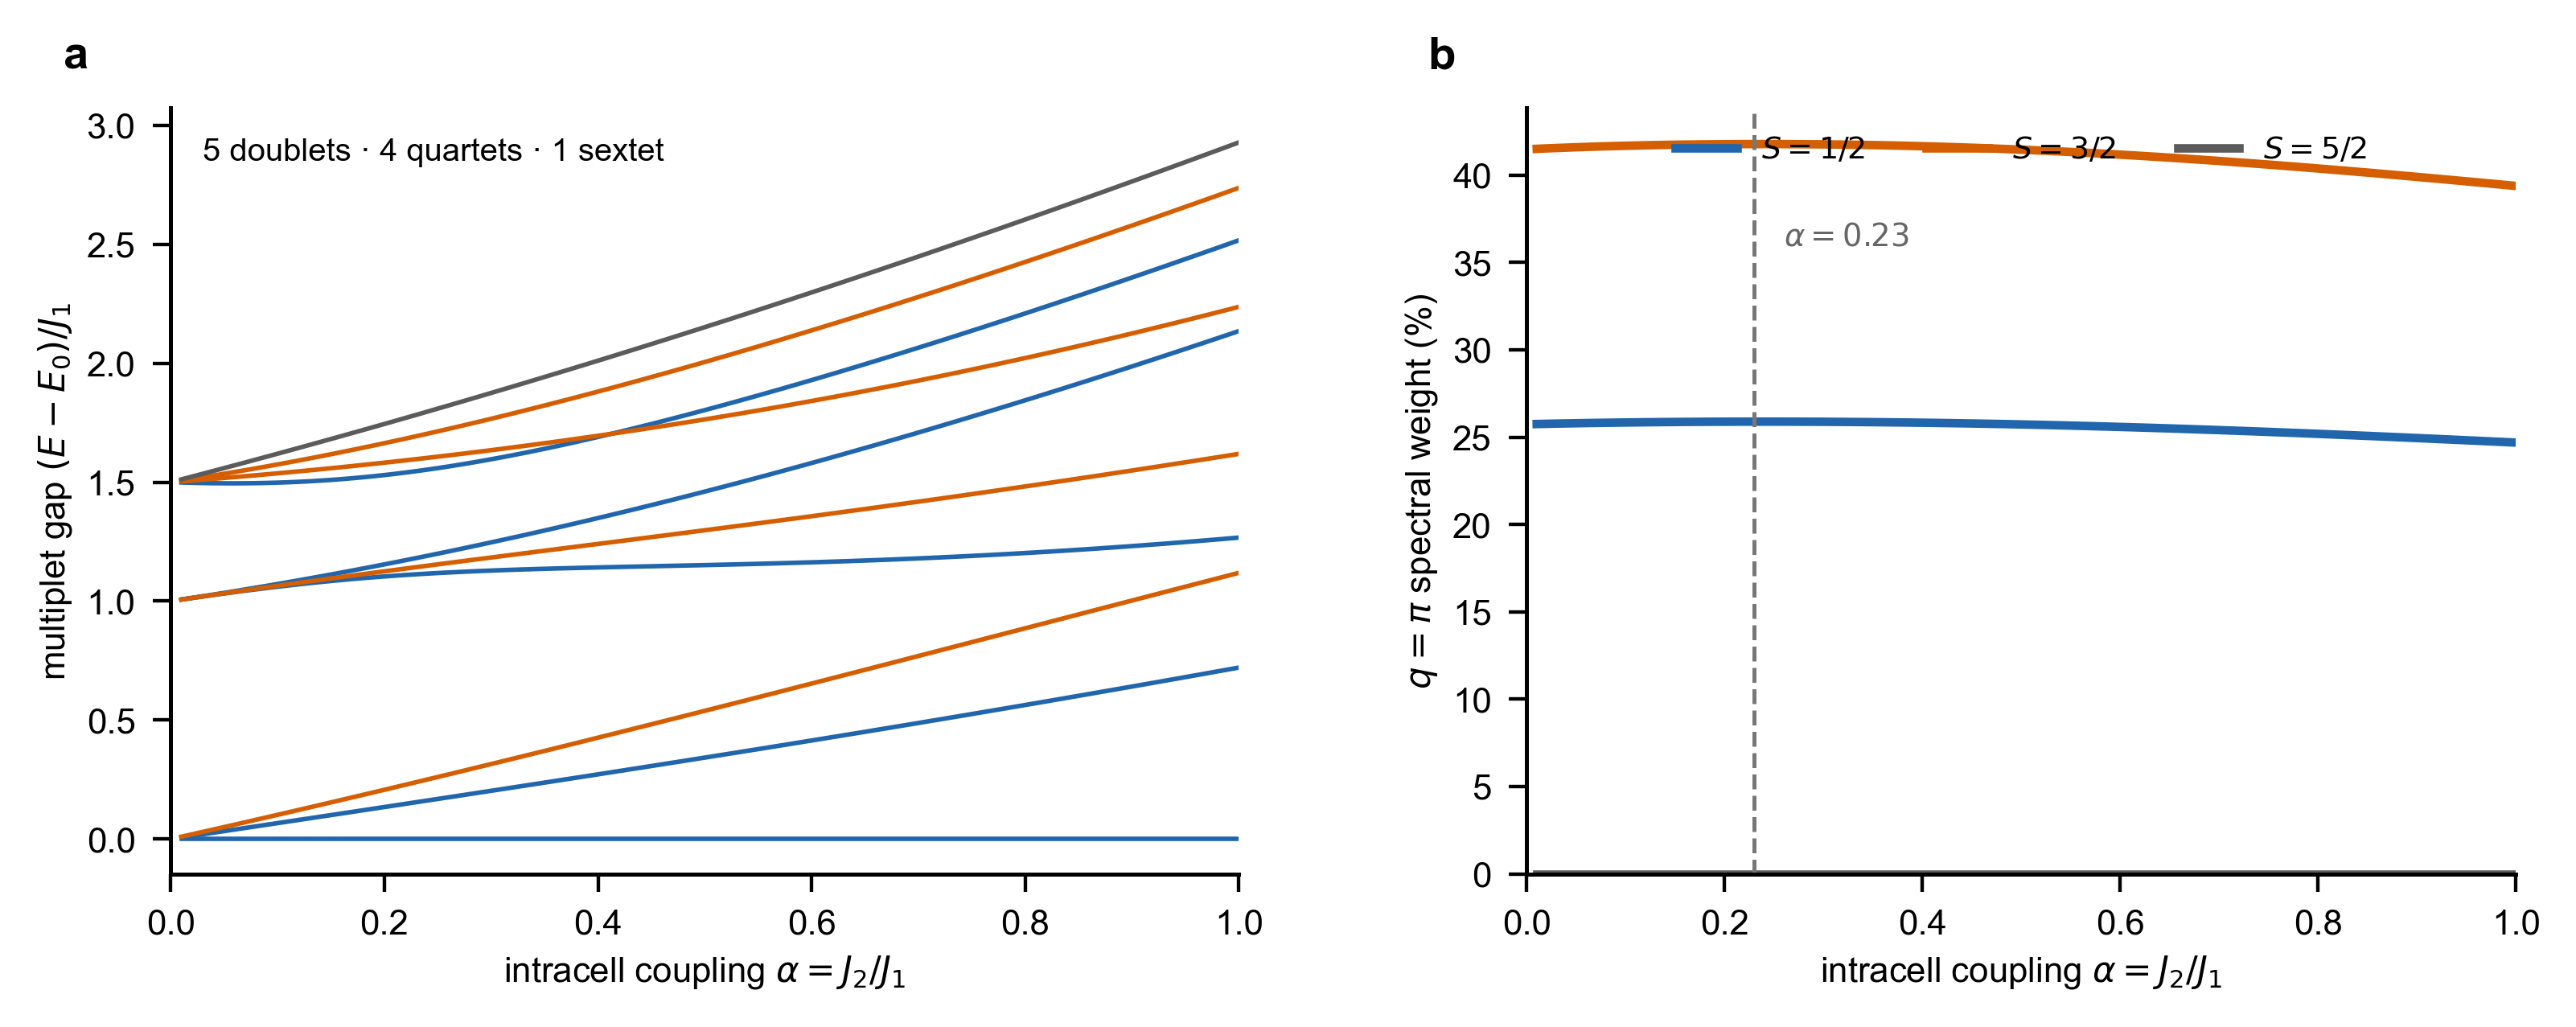
\includegraphics[width=\textwidth]{fig2_multiplet_parity.png}
  \caption{Multiplet flow and the $q=\pi$ parity filter for positive $\alpha$.
  The lowest excited doublet is dark, whereas even-parity spin-$3/2$ multiplets dominate the local inelastic response.}
  \label{fig:multiplets}
\end{figure*}

\subsection{Positive couplings support one resolved effective-chain regime}

The strict positive-region mesh contains 105 accepted records.
Its $L=40,60,80$ finite-size diagnostic does not produce a stable interior crossing.
All accepted interior size differences retain the same sign under leave-one-out and weakest-point audits.
This bounded negative result establishes that the present data resolve no internal boundary in $0\leq\alpha,\beta\leq1$, but it does not prove that every thermodynamic point belongs to one phase.

At $\alpha=0.23$ and weak inter-cell coupling, matched-size entanglement estimators give $\ceff=1.0240$--1.0331 relative to an open spin-$1/2$ Heisenberg-chain oracle.
The comparison uses open chains of $N=8$--$24$ pentamers ($L=40$--$120$) with the same boundary condition and fitting window for both models, and the bond entropy is stable against a doubling of the retained bond dimension (largest relative change $2.4\times10^{-4}$).
Finite-size spin gaps extrapolate close to zero, the correlation envelope has exponents 0.95--0.98, and the static structure factor is dominated by $q=\pi$.
Together, these observables are consistent with a gapless antiferromagnetic effective chain at the tested points~\cite{descloizeaux1962_verified}.
The unmatched absolute $\log L$ fits do not pass an independent quality gate, so the calibrated matched-size ratio is the operative statement; we do not report an unbiased thermodynamic central charge.

\begin{figure*}[t]
  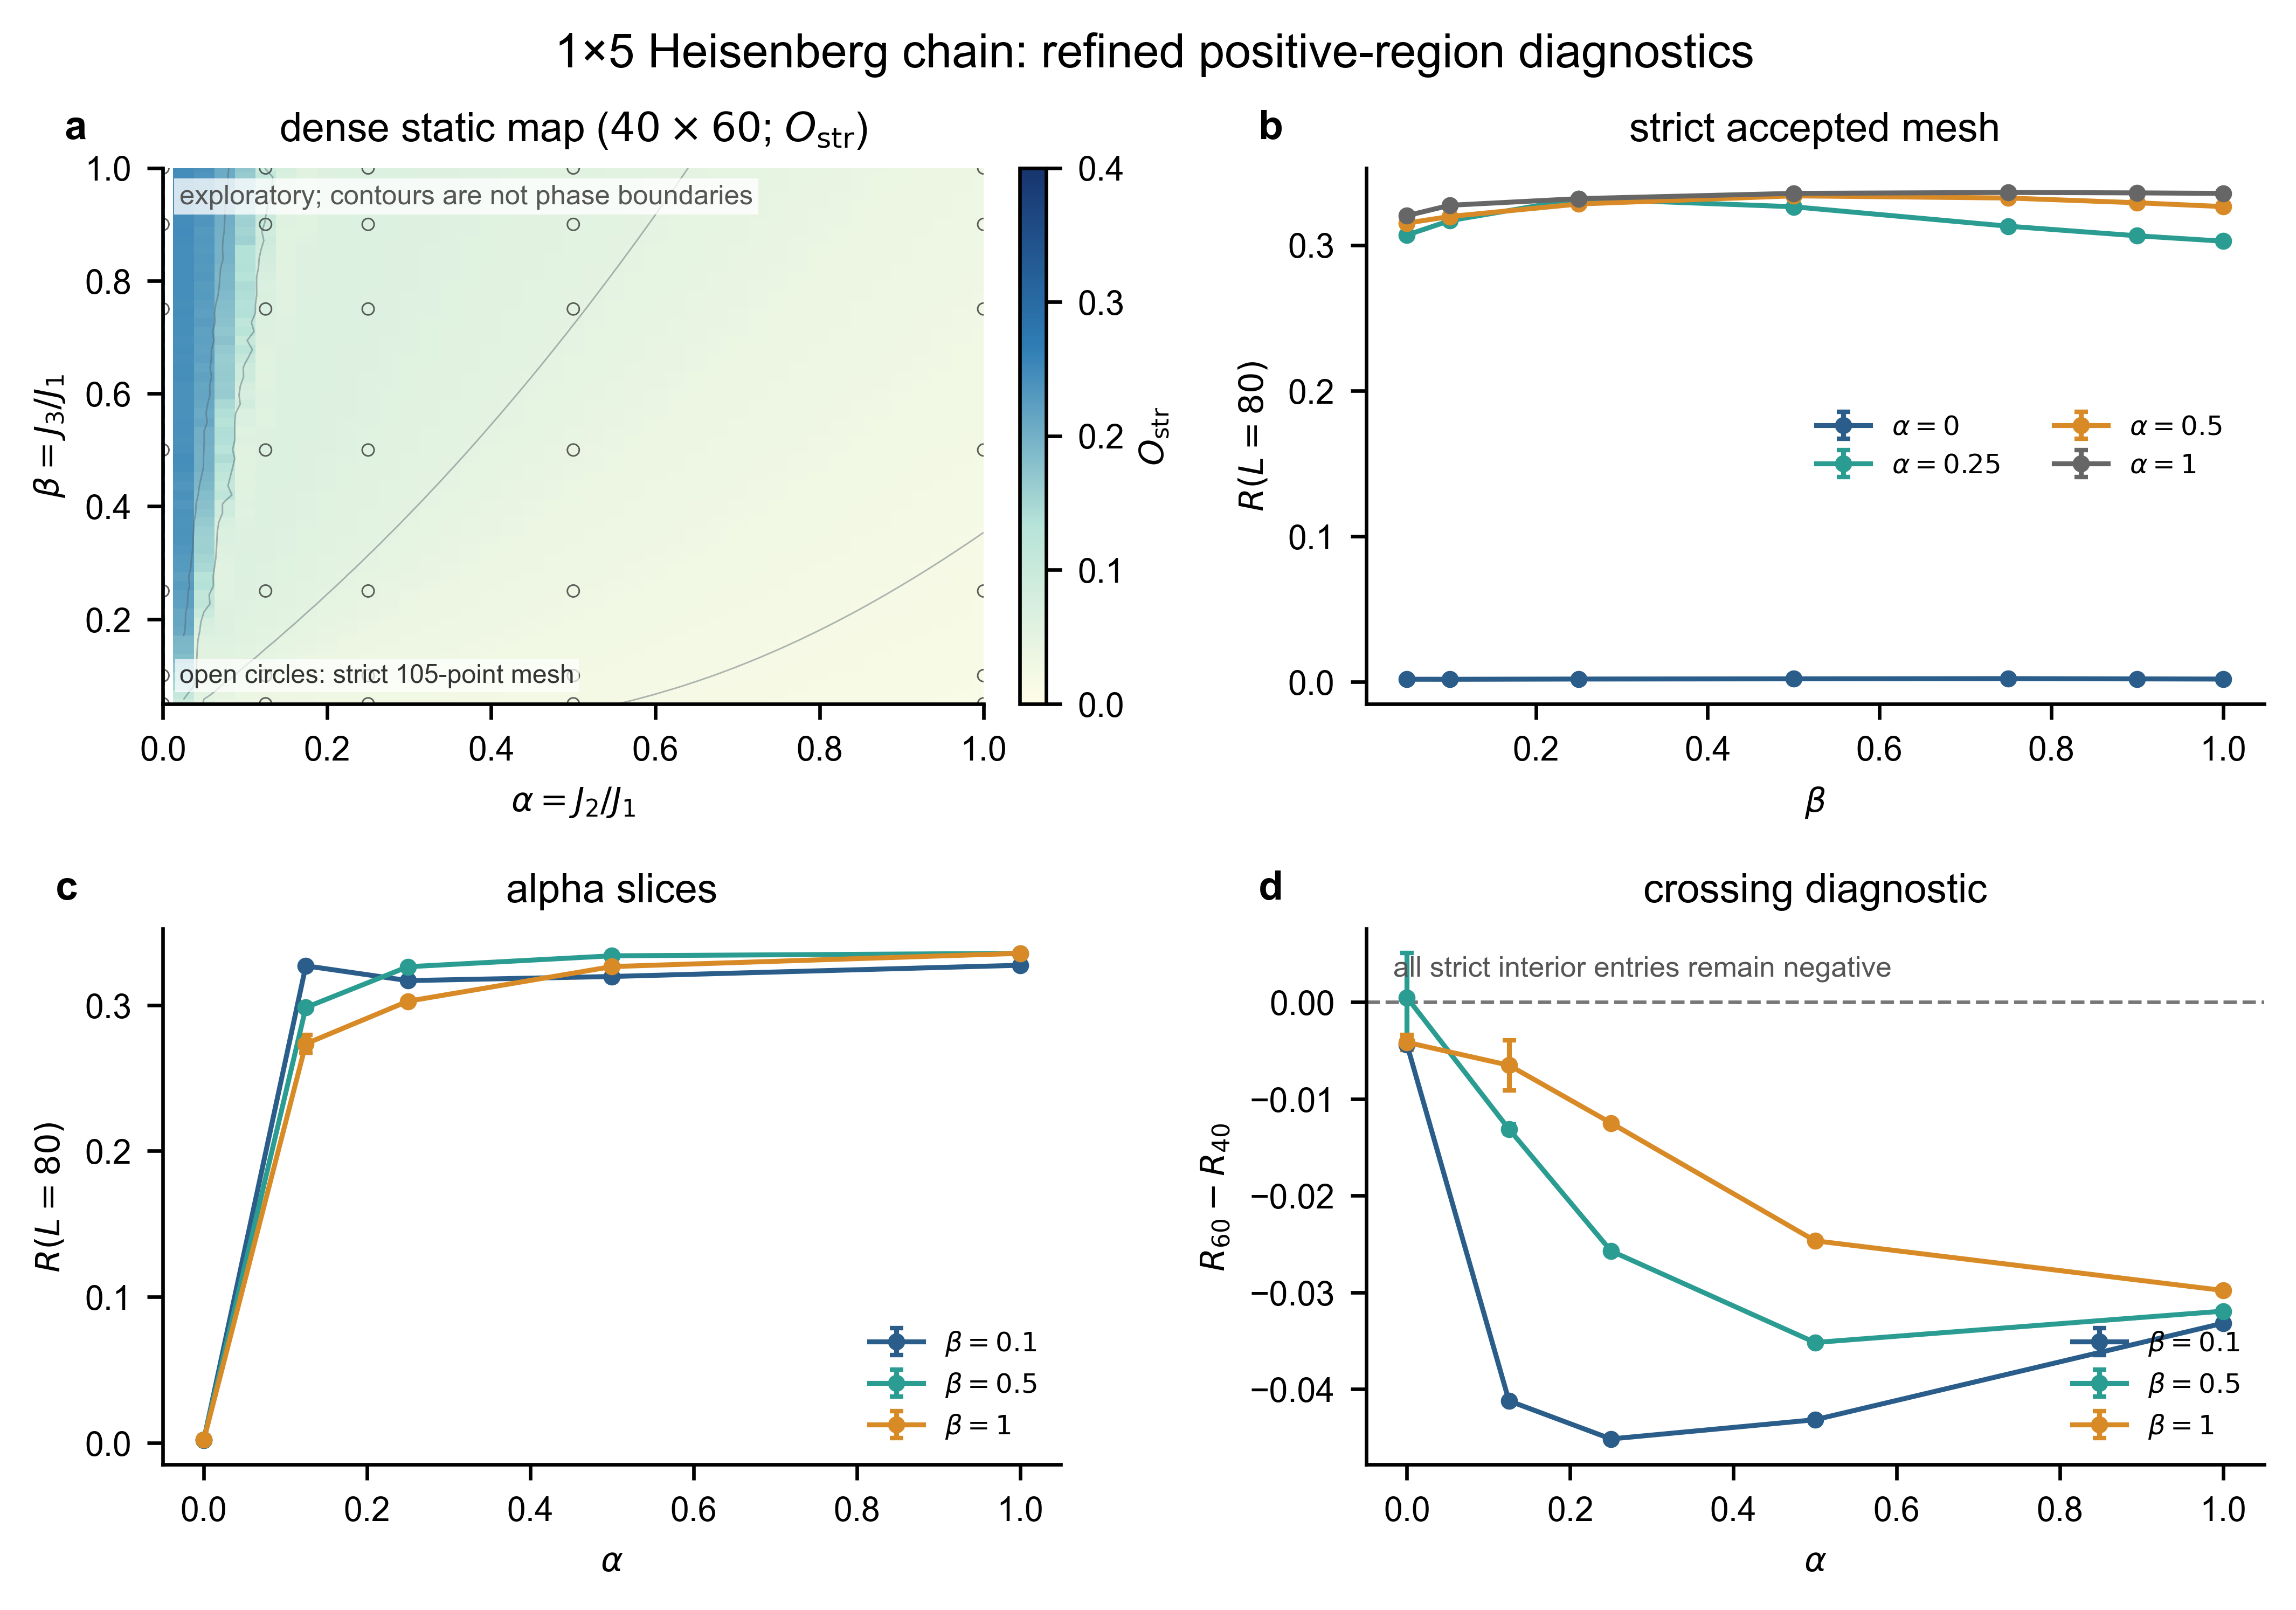
\includegraphics[width=0.98\textwidth]{fig3_positive_static.png}
  \caption{Positive-region ground-state diagnostics.
  The dense map is exploratory, whereas the strict 105-record $L=40,60,80$ mesh supplies the accepted crossing test.
  No stable internal bracket is resolved.}
  \label{fig:positive-static}
\end{figure*}

\begin{figure*}[t]
  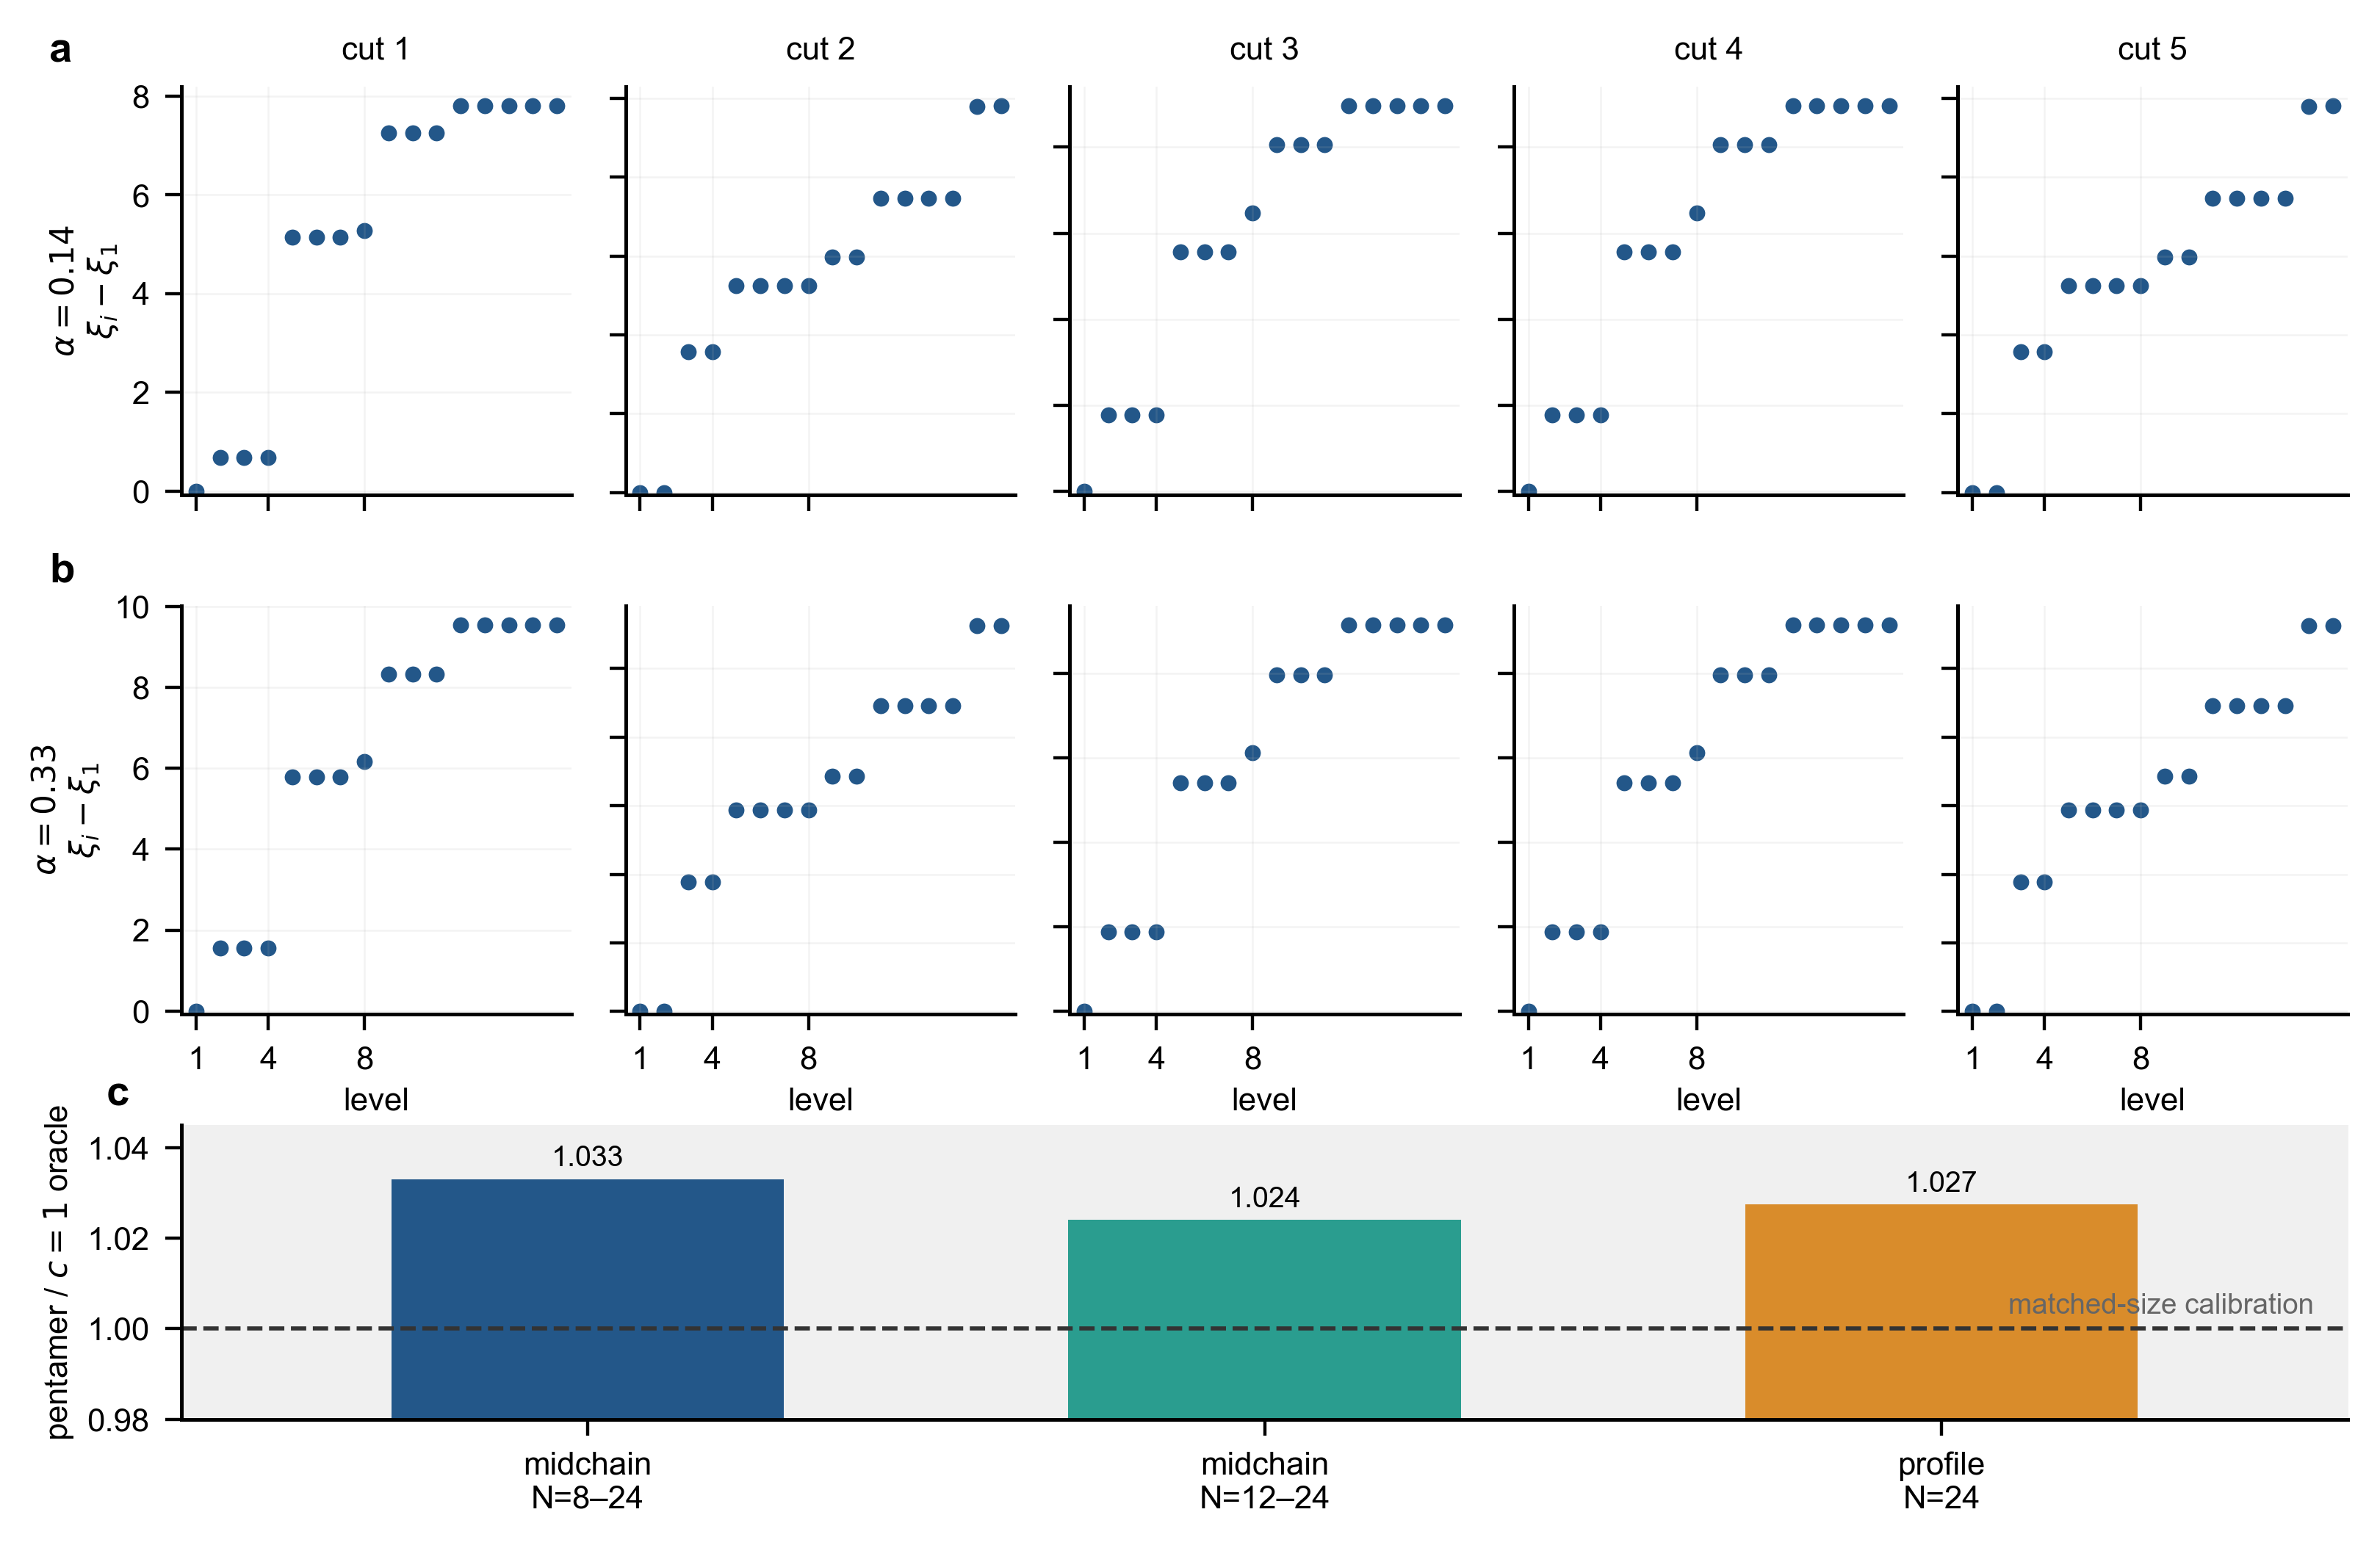
\includegraphics[width=0.94\textwidth]{fig4_entanglement.png}
  \caption{Entanglement and finite-size low-energy diagnostics.
  Five inequivalent bond classes are calibrated against a matched-size $c=1$ Heisenberg-chain oracle.
  The coefficient is interpreted only at the tested points.}
  \label{fig:entanglement}
\end{figure*}

\subsection{Reflection parity selects the visible local excitation}

The lowest excited doublet is not the lowest visible $q=\pi$ excitation.
Its projector-resolved spectral weight is below $4.6\times10^{-27}$ at the three representative positive-$\alpha$ points because the $q=\pi$ spin operator is even under reflection, whereas the target doublet is odd.
The lowest even-parity spin-$3/2$ multiplet carries weight 0.325--0.333, and all spin-$3/2$ multiplets together account for $84.1\%$--$97.6\%$ of the isolated-pentamer inelastic response.
This result identifies which local sector can contribute when collective states form, without assuming that the isolated multiplet remains a sharp quasiparticle at finite $\beta$.

\begin{figure*}[t]
  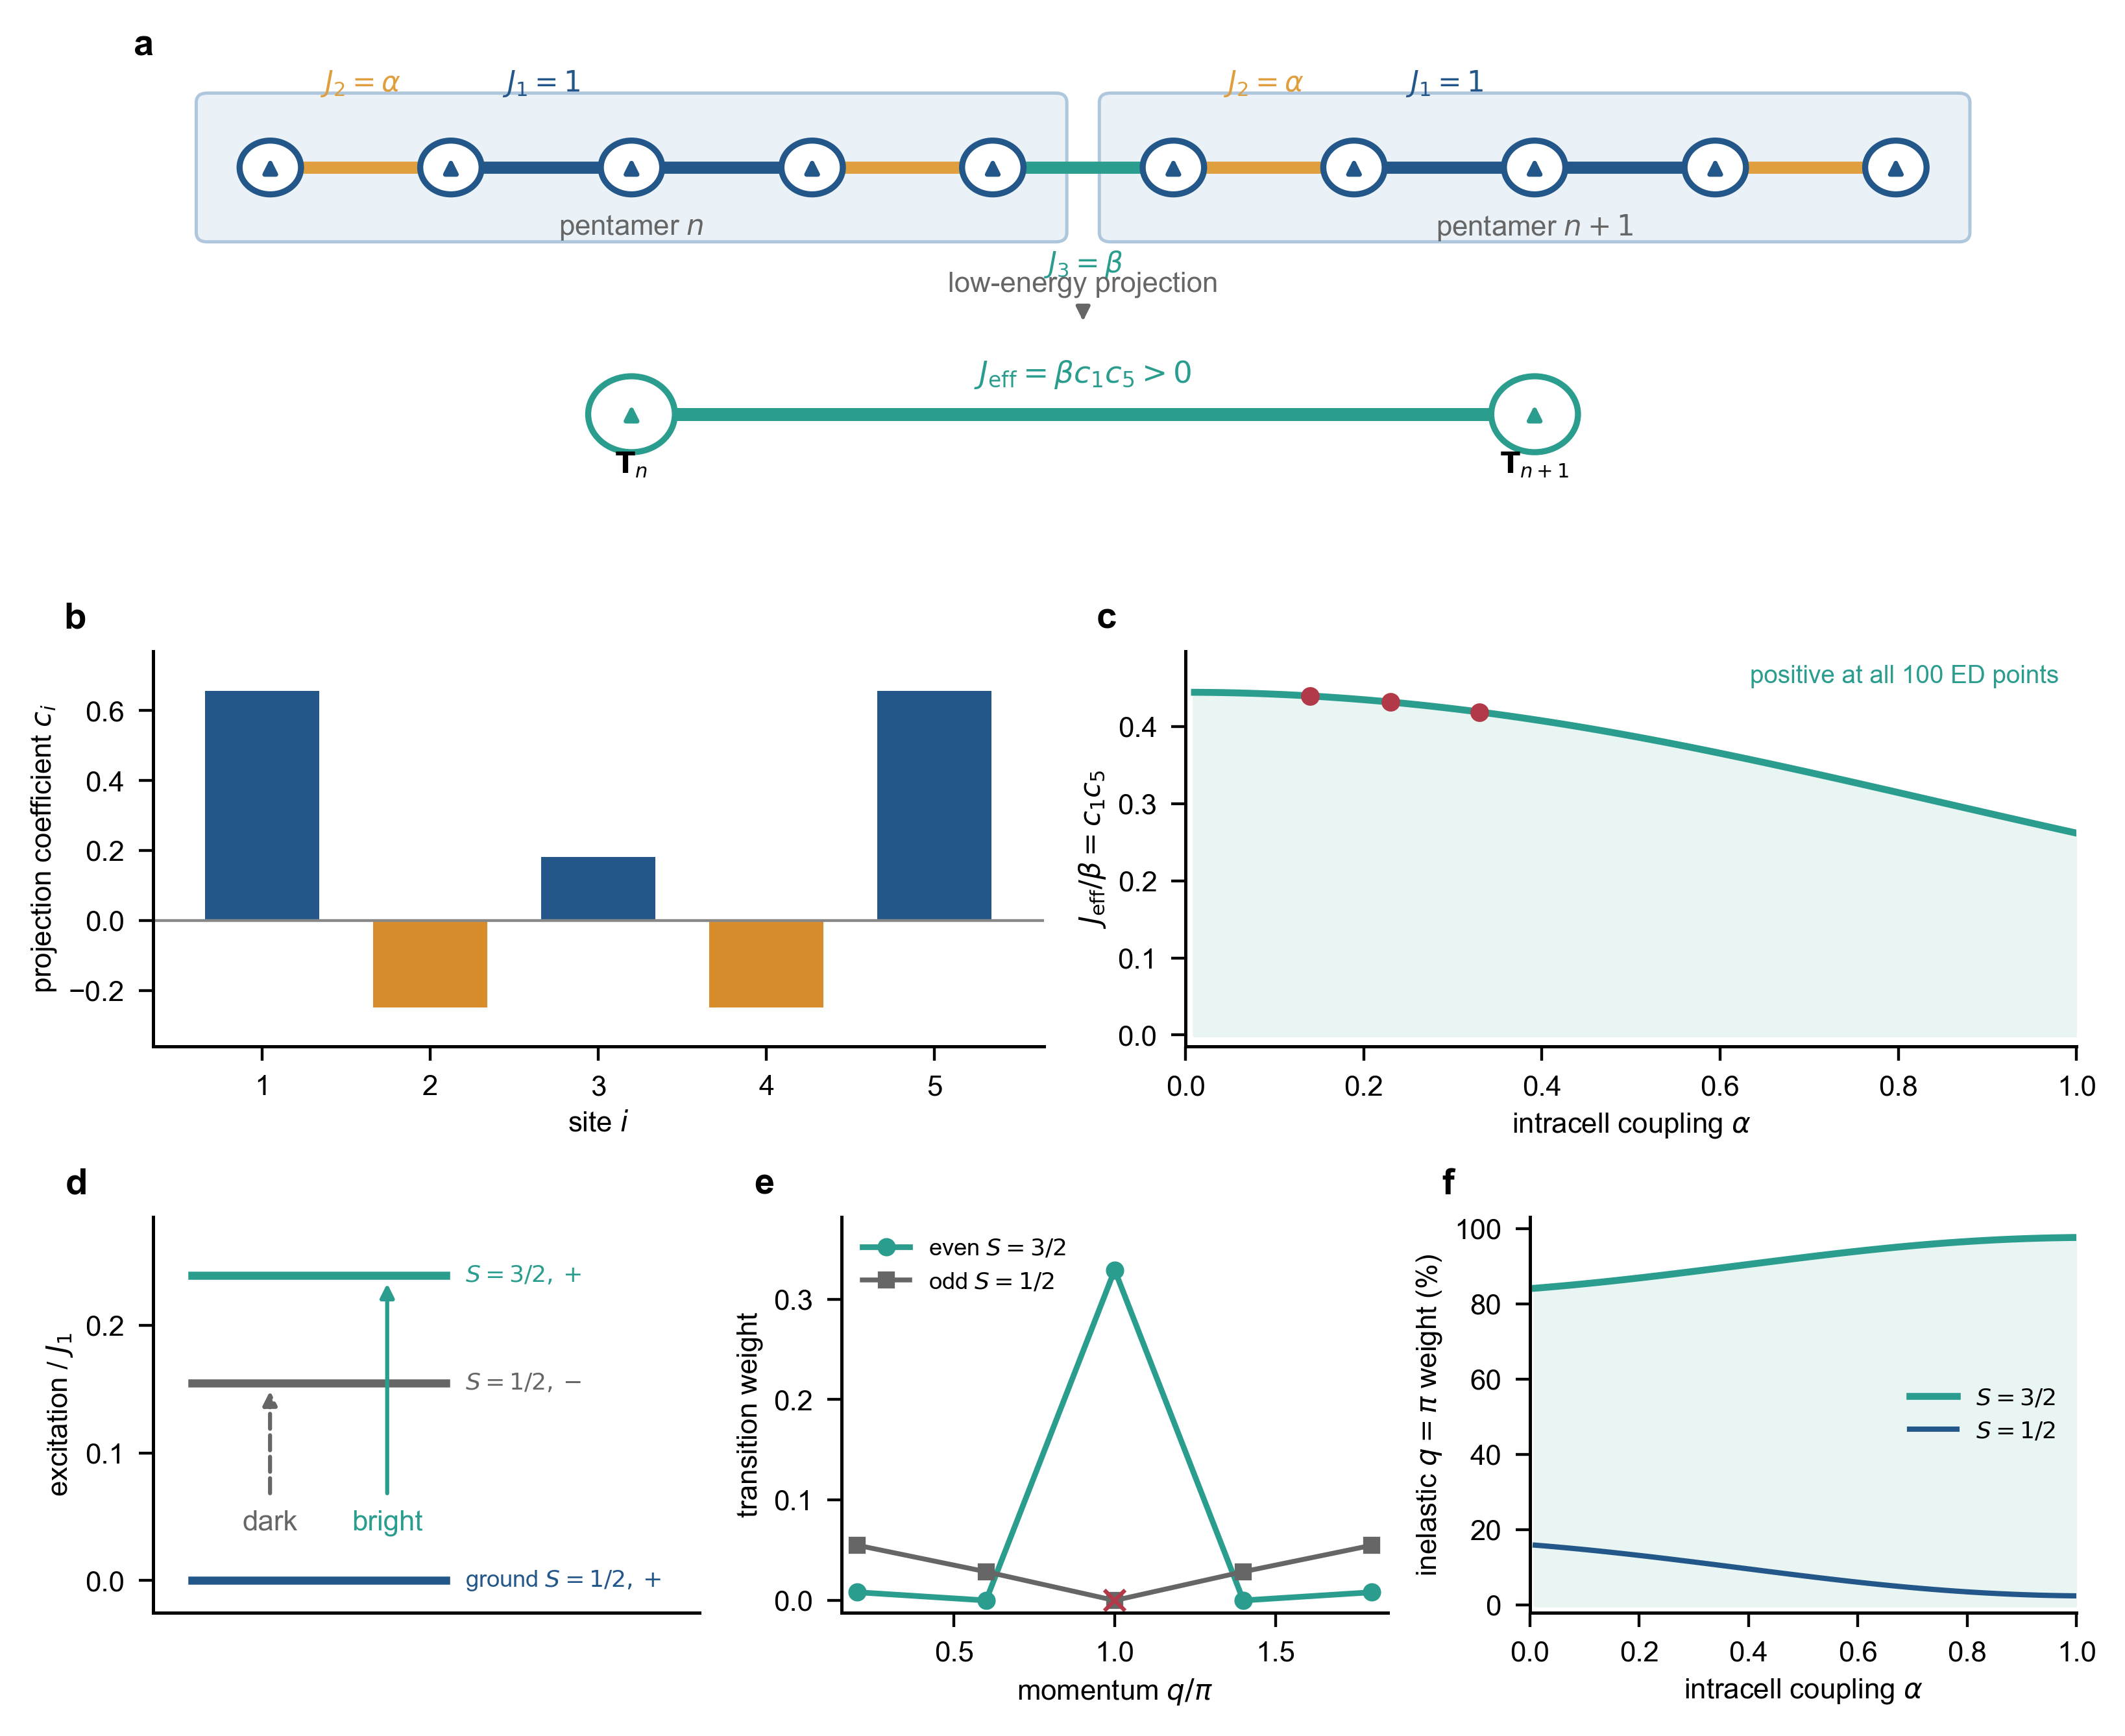
\includegraphics[width=0.92\textwidth]{fig5_selection_rules.png}
  \caption{Effective-chain continuum and local selection rules.
  The continuum bounds describe the weak-coupling effective chain, while the isolated-pentamer weights identify bright local spin-$3/2$ channels without assigning an unvalidated quasiparticle label.}
  \label{fig:selection}
\end{figure*}

\subsection{Collective dynamics confirms the pointwise spectral picture}

At $(\alpha,\beta,L,q)=(0.23,0.5,40,\pi)$, eleven accepted correction-vector frequencies cover $0\leq\omega/J_1\leq1.5$ and pass the peak-bracketing, spectral-weight, and residual gates.
The line shape agrees with the independently converged time-evolution result within the declared peak-position and integrated-weight budgets.

Full-momentum time evolution was completed at $(\alpha,\beta)=(1,1)$, $(1,0.1)$, and $(0.23,0.5)$.
All six individual runs and all three $\Delta t$/$\Delta t/2$ pairs passed.
The global and $q=\pi$ peak drifts are 0, 0, and $0.01J_1$ for the uniform, weak-coupling, and agreement points.
The corresponding low-frequency integrated-weight changes are $4.32\times10^{-5}$, $2.74\times10^{-5}$, and $1.97\times10^{-5}$.

The uniform point uses broadening $\eta=0.1$, whereas the weak-coupling and agreement points use $\eta=0.2$; all three use a spatial window of 18 sites.
We compare the spectral organization and time-step stability but do not compare weak-peak linewidths across different broadenings.

\begin{figure*}[t]
  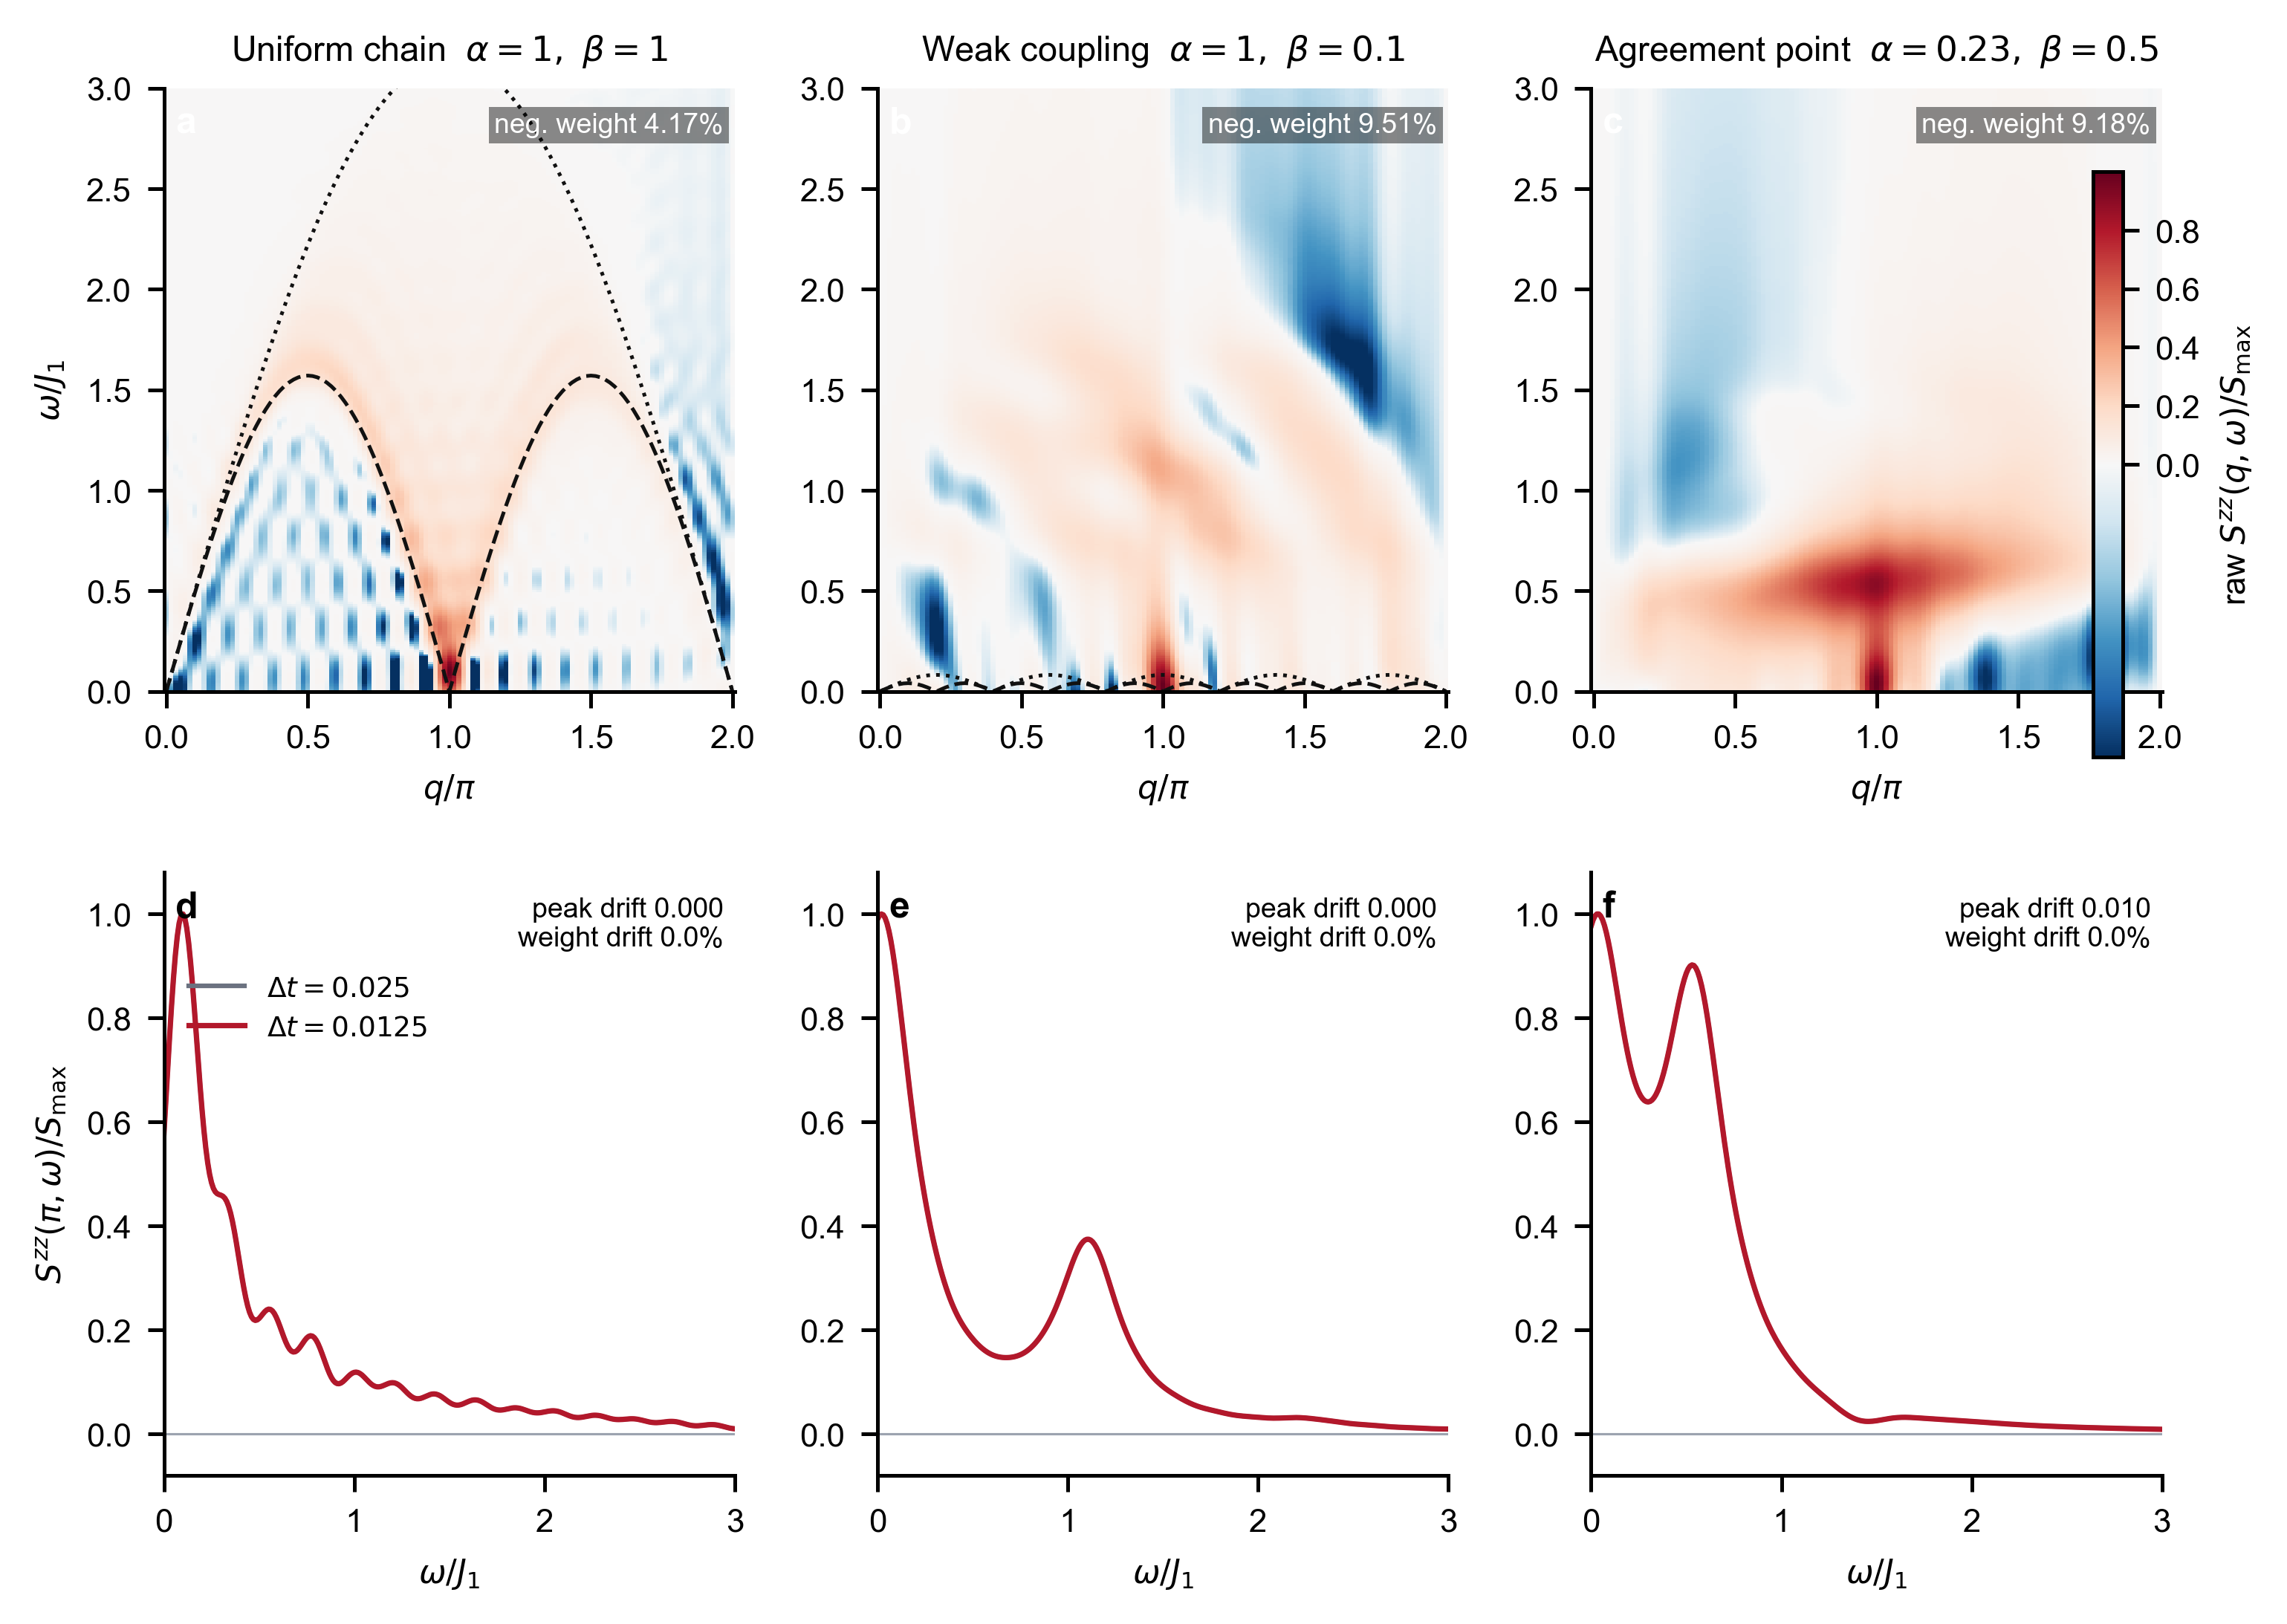
\includegraphics[width=0.97\textwidth]{fig6_fullq_dynamics.png}
  \caption{Raw full-momentum $\Szz$ and paired $q=\pi$ time-step slices at three representative positive-coupling points.
  Negative Fourier ringing is shown rather than clipped.
  All six runs and all three $\Delta t$/$\Delta t/2$ pairs pass the spectral gates.}
  \label{fig:fullq}
\end{figure*}

\begin{figure}[t]
  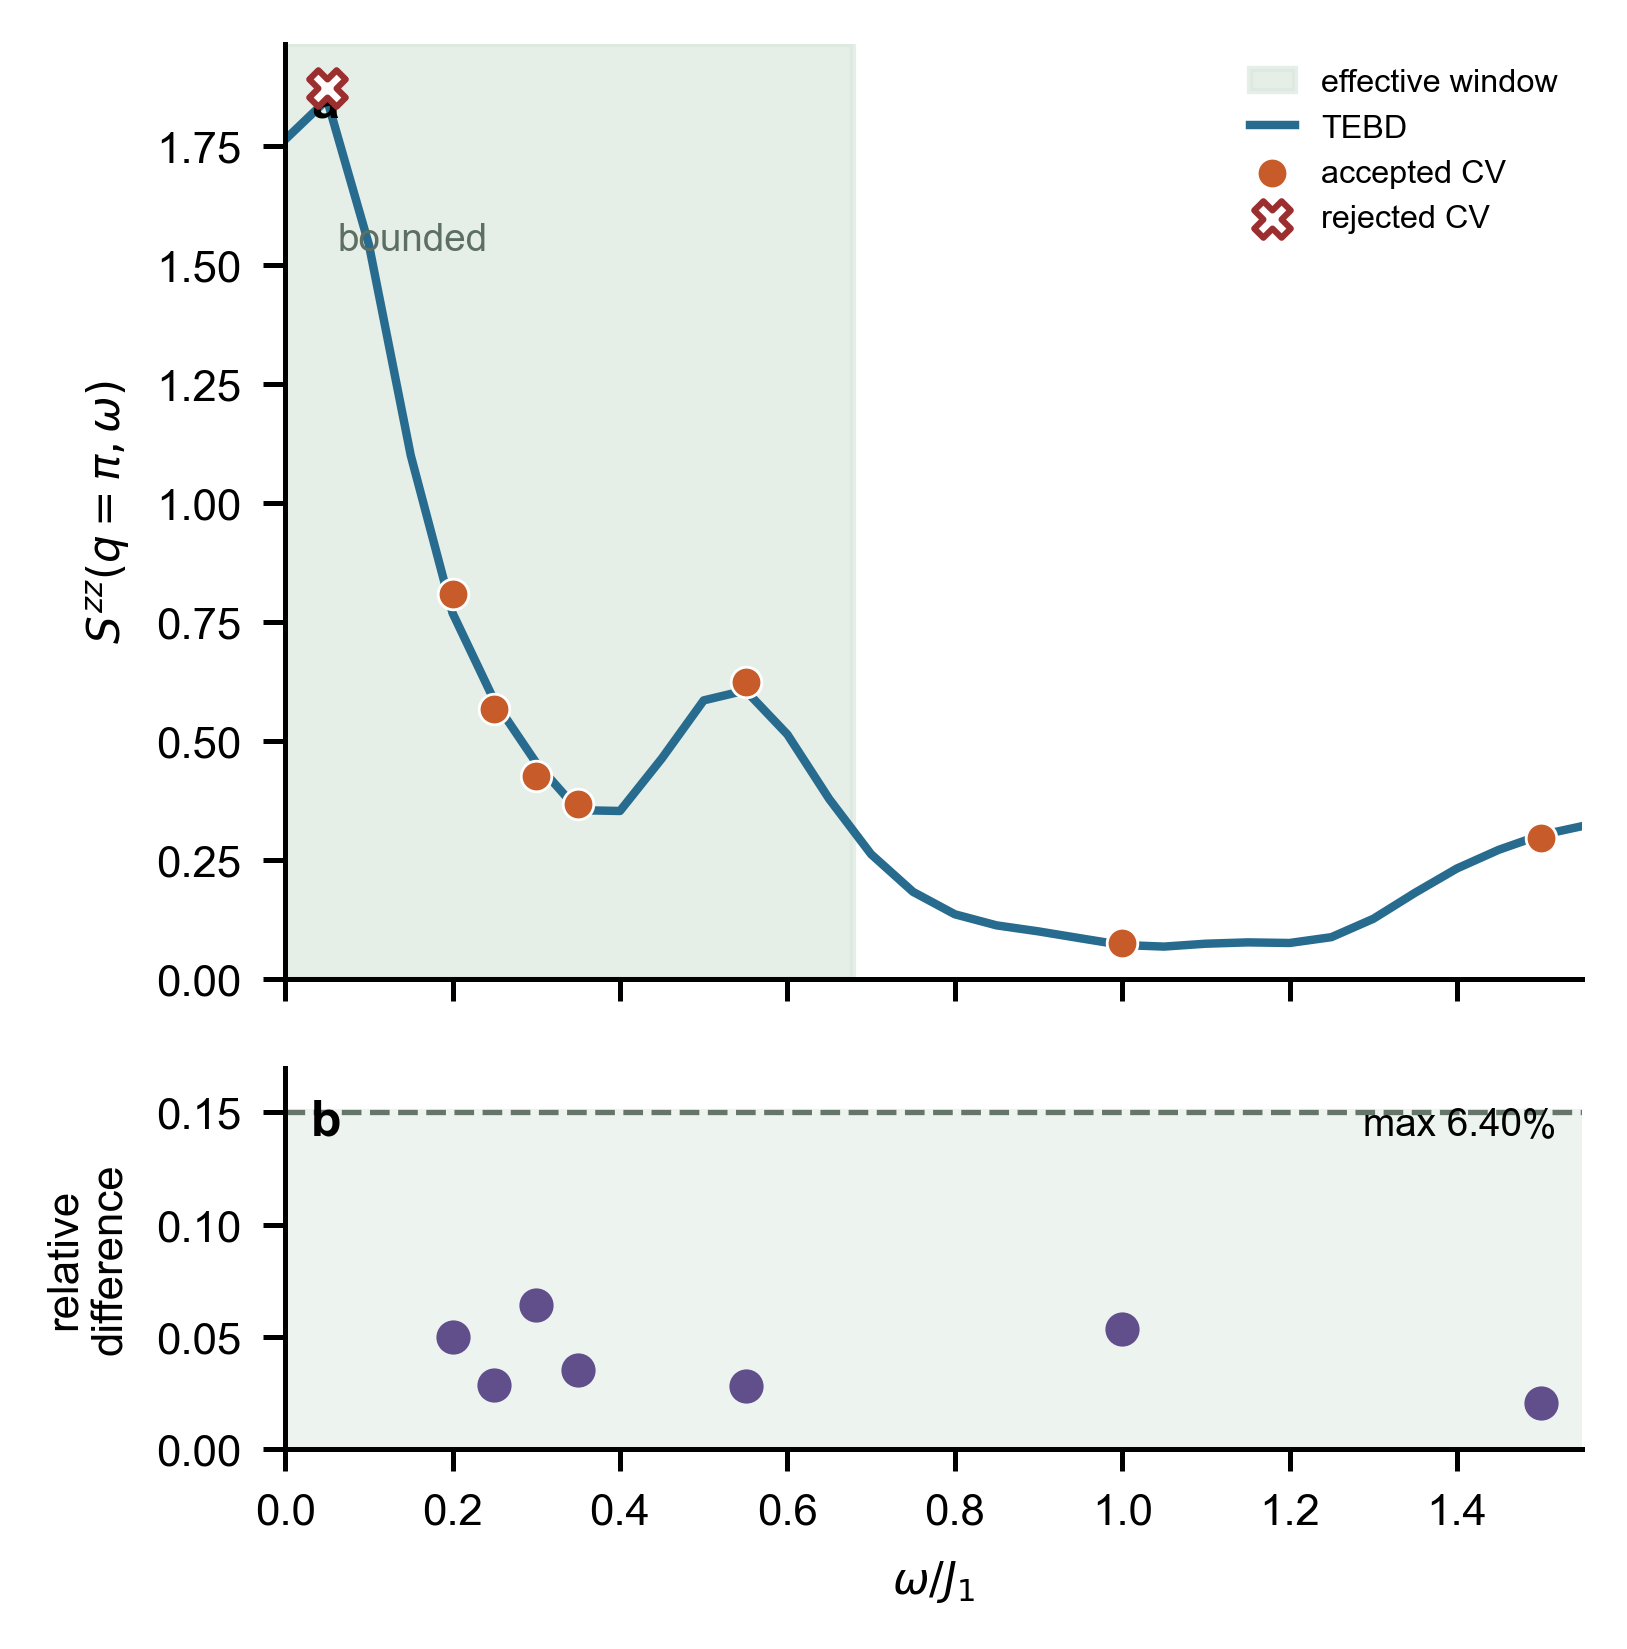
\includegraphics[width=\columnwidth]{fig7_cv_tebd.png}
  \caption{Pointwise correction-vector and time-evolution comparison at $\alpha=0.23$, $\beta=0.5$, $L=40$, and $q=\pi$.
  Eleven accepted frequencies bracket the principal feature and cover $0\leq\omega/J_1\leq1.5$.}
  \label{fig:cv-tebd}
\end{figure}

\subsection{Negative intra-cell exchange reconstructs the finite-size momentum}

The negative-$\alpha$ data show a reproducible change in the dominant structure-factor momentum.
Deep in the scanned region, $\qpeak\simeq0.60\pi$; closer to $\alpha=0$, the maximum locks to $q=\pi$.
The local multiplet structure offers a candidate explanation for the deep-region value.
At all 201 sampled points with $-1\leq\alpha\leq-0.001$, the isolated pentamer has a spin-$3/2$ ground multiplet rather than the spin-$1/2$ doublet found for $\alpha>0$.
Projecting the intra-cell couplings onto that quartet and evaluating the single-spin shape factor at three representative momenta gives a positive effective exchange $\Jeff/\beta=0.1075$--$0.1111$, with the $q=0.60\pi$ weight in the range 0.62--0.73 while the $q=\pi$ weight never exceeds $1.3\times10^{-2}$ on the same scale.
The projector identities are satisfied to $3.1\times10^{-16}$ and the dominant folded momentum is $0.60\pi$ without exception.
This is a local single-cell statement: it shows that the deep-region momentum scale is already selected by the isolated quartet, but it does not establish that the chain orders there.

Stage B evaluated 96 parameter--size records at 48 coupling points.
Eighty-nine records passed the Practical V2 gates, while seven non-boundary records remained bounded and were excluded from accepted-only inference.

The accepted-only analysis identified eight candidate intervals across seven $\beta$ slices.
Stage C evaluated these intervals with 29 additional $L=60,80$ cells at 64 sweeps.
All 29 cells passed the remote parent and child checksums, non-overwriting transfer, local checksum, and independent validator.
Seven of eight targets retain either a momentum reconstruction or a sign change in $\Delta R=R_{80}-R_{60}$ that satisfies its declared diagnostic criterion.
No adjacent interval carries both signatures.
Only the $\beta=0.05$ momentum interval reaches the target width 0.025, and the $\beta=0.10$ slice supplies no supported internal interval at the final size pair.

The data establish a finite-size momentum reconstruction but do not locate a joint thermodynamic boundary.
The mismatch is compatible with a broad crossover, a slowly converging incommensurate regime, or residual finite-size effects.

\begin{figure}[t]
  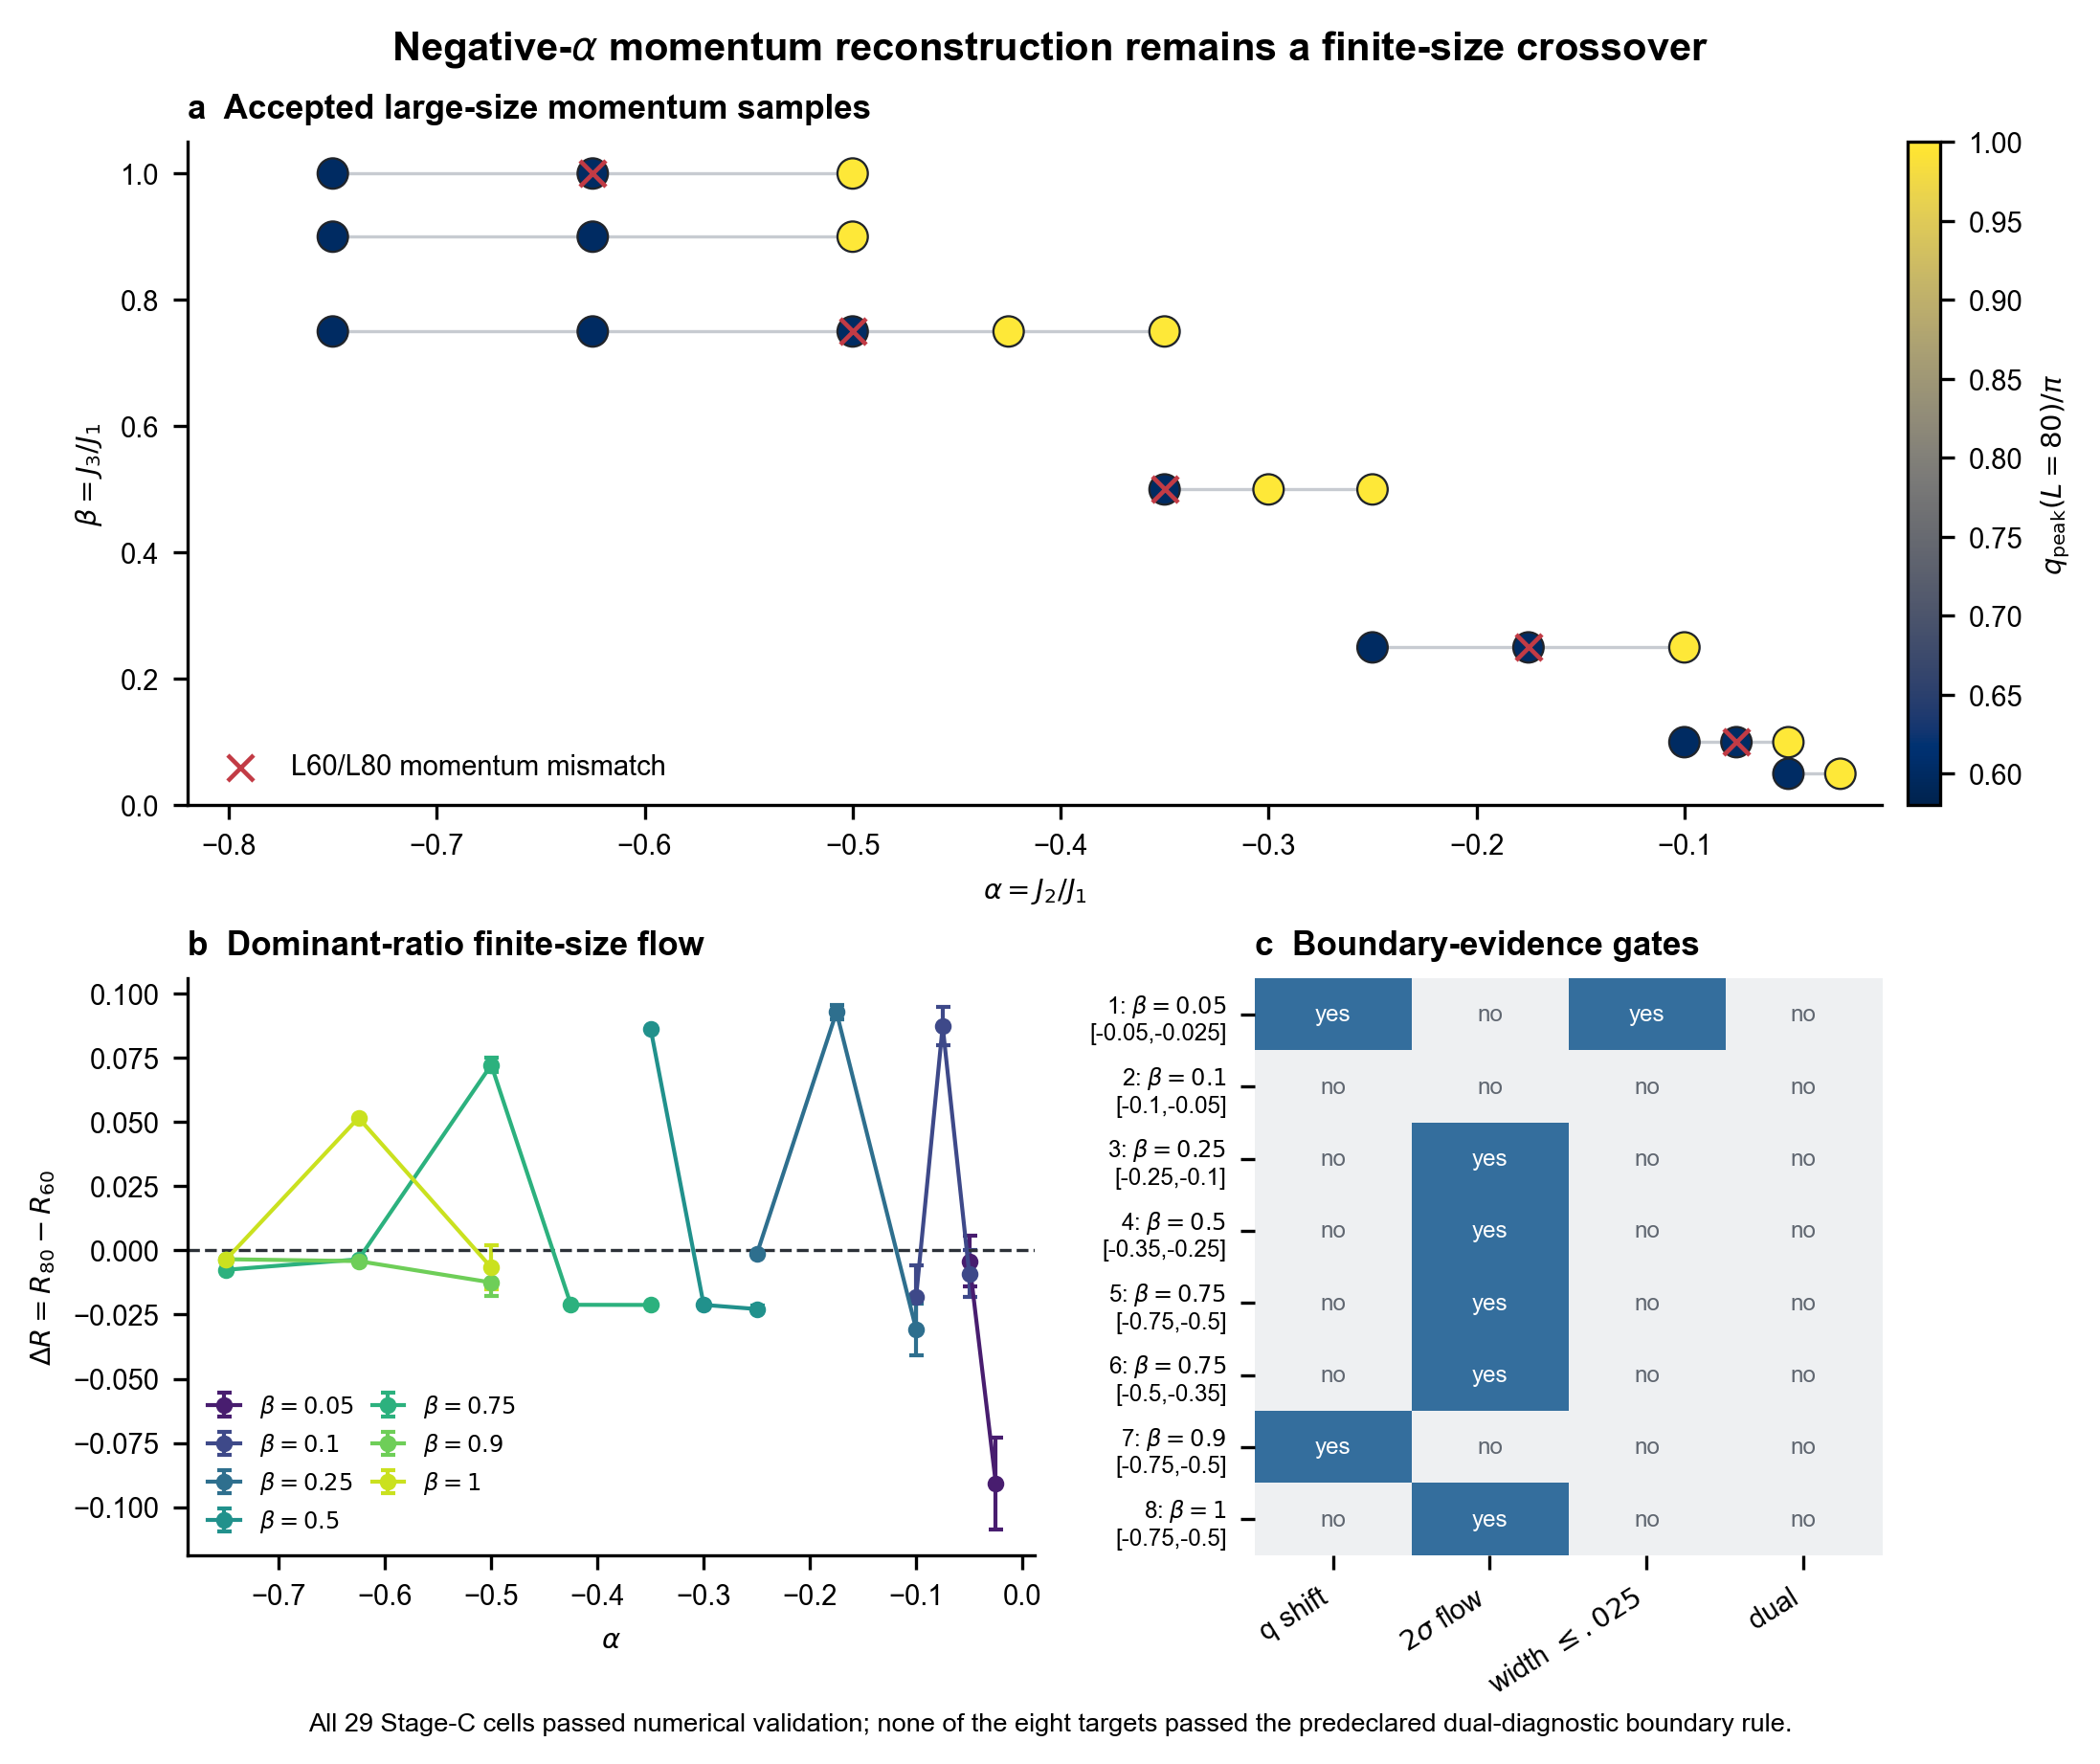
\includegraphics[width=\columnwidth]{fig8_negative_reconstruction.png}
  \caption{Accepted-only negative-$\alpha$ momentum reconstruction.
  Large-size data move from $\qpeak\simeq0.60\pi$ to $\pi$, but the momentum and dominant-ratio diagnostics do not select the same adjacent interval.}
  \label{fig:negative-reconstruction}
\end{figure}

\subsection{Saved-state diagnostics and terminal solver control}

Six additional points were evaluated with saved $L=80$ ground-state wavefunctions using two $S^z=0$ initial states and 64 sweeps per initial state.
The points were $\alpha=-0.25,-0.175,-0.10$ at $\beta=0.25$ and $\alpha=-0.625,-0.50,-0.425$ at $\beta=0.75$.
All parent runs passed the Practical V2 gates, with a largest variance per site of $1.2875\times10^{-9}$.

At $\beta=0.25$, the earlier $L=80$ audit gave $\ceff=0.467$--0.605 at $\alpha=-0.10$, compared with 0.886--0.971 at $\alpha=-0.175$ and 0.981--1.049 at $\alpha=-0.25$.
The three $\beta=0.75$ points gave 0.905--0.976.
These ranges measure sensitivity to the fitting window and initialization; they are not confidence intervals.

A subsequent size comparison used $L=40,60,80$ at $\alpha=-0.175,-0.150,-0.125,-0.100$ and $\beta=0.25$.
At $\alpha=-0.10$, the ten-intercept coefficients span 0.970--1.340, 0.625--0.959, and 0.467--0.605 with increasing length.
At fixed window $f=0.20$, the dual-start mean decreases from 0.988 to 0.695 and 0.533.
That decrease, however, is not a converged finite-size trend.
The whole sequence was computed with the historical Krylov setting, and only its $L=80$ endpoint has a $k=8$ control.
At that point the period-10, $f=0.20$ coefficient moves from 0.582 to 0.932 (\texttt{center}) and from 0.484 to 0.932 (\texttt{ferro\_j2}), after which the two initial states agree to $3.4\times10^{-8}$.
A solver setting that shifts an endpoint by this amount cannot support a size-scaling reading of the sequence, and the $L=40$ and $L=60$ records have no equivalent control.

\begin{figure}[t]
  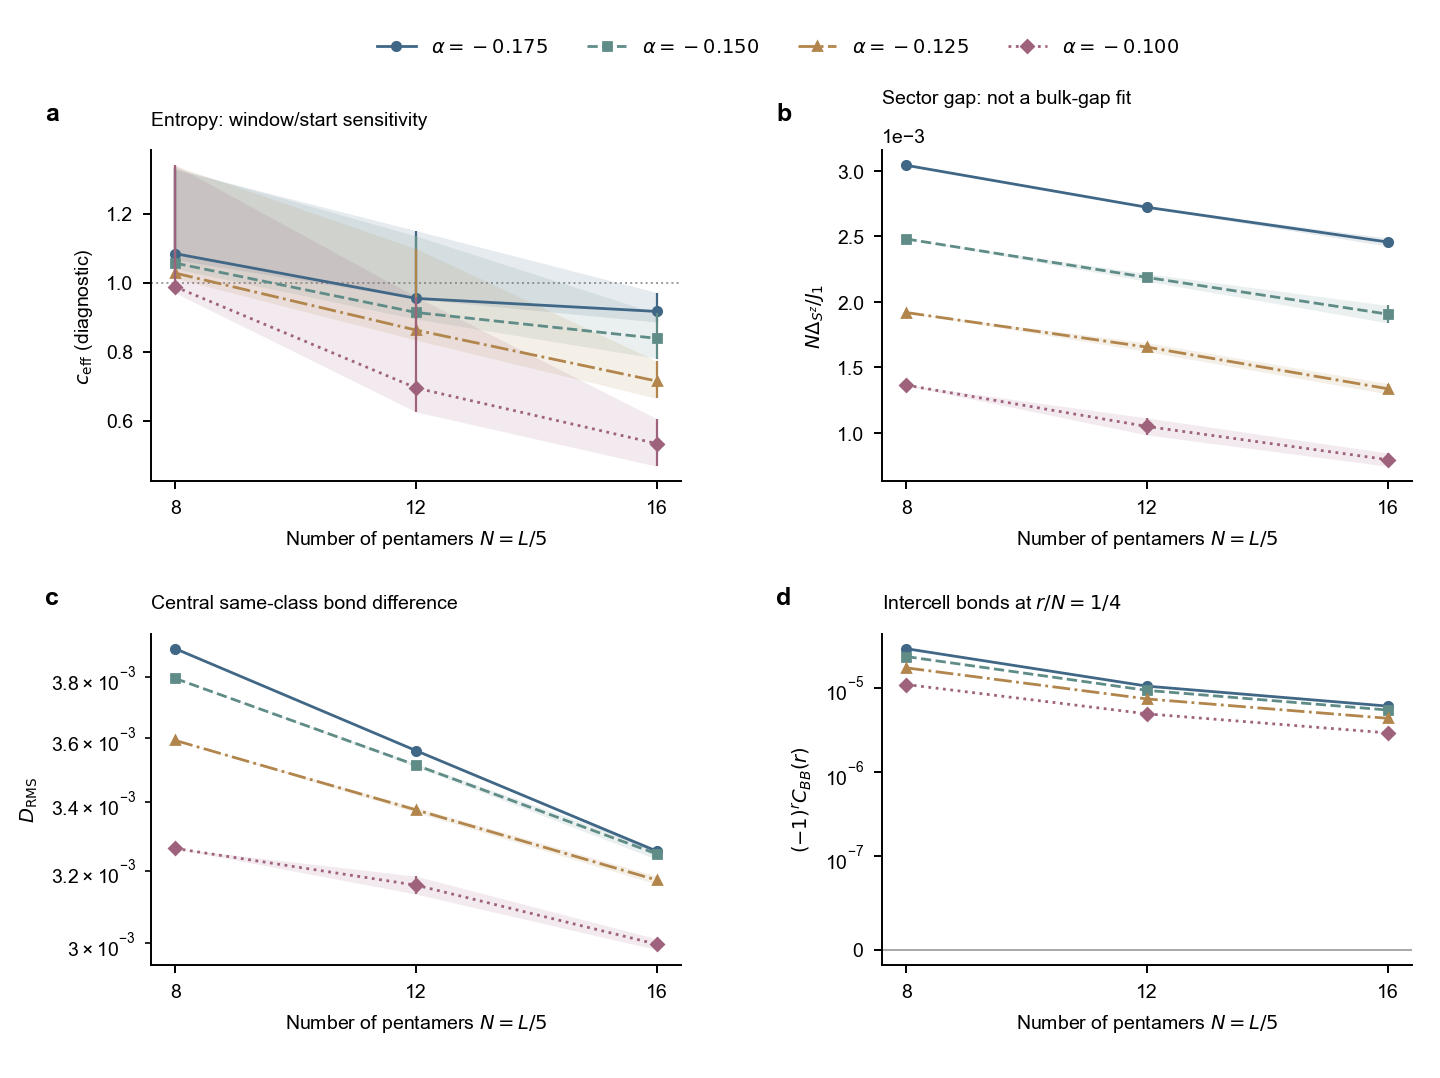
\includegraphics[width=\columnwidth]{fig9_negative_size_evidence.png}
  \caption{Joint finite-size evidence near the negative-$\alpha$ anomaly.
  Entropy coefficients, bond-class variation, connected correlations, and sector gaps are shown together to expose size and initialization sensitivity.
  All panels use the historical solver setting; the $k=8$ control applies only to the $L=80$, $\alpha=-0.10$ endpoint and is not propagated through this figure.}
  \label{fig:negative-size}
\end{figure}

The terminal Krylov control identifies which part of this anomaly was numerical.
The earlier $k=3\rightarrow8$ change strongly revised some entropy slopes at $\alpha=-0.10$, showing that the old solver setting was not stable.
By contrast, the final $k=8\rightarrow12$ comparison at the same $L=80$ point is stable to the small absolute differences reported in Sec.~\ref{sec:methods} and leaves $\qpeak=\pi$.
This makes the accepted $L=80$ observables at that point robust against a further increase of the Krylov subspace.
It does not supply a $\chi$ series, larger sizes, or a thermodynamic order parameter.

\section{Discussion}
\label{sec:discussion}

\subsection{Contrast with the tetramer chain}

The main contrast with the reference tetramer follows from unit-cell parity.
Four spin-$1/2$ degrees of freedom can form an integer-spin or singlet cluster sector.
Five leave a half-integer degree of freedom unless translation symmetry is broken or the ground state is degenerate.
At the tested positive-$\alpha$ pentamer points, the surviving doublet converts the inter-cell exchange into an antiferromagnetic interaction between effective spins.
The finite-size data are therefore consistent with a critical effective chain, whereas tetramer phase names and its local triplon, quarton, or higher composite labels cannot be transferred by geometric analogy alone~\cite{li2026tetramer_verified}.

The spectral comparison sharpens this distinction.
The pentamer's odd-parity excited doublet is dark at $q=\pi$, while higher even-parity spin-$3/2$ sectors remain bright.
In the chain, that local hierarchy coexists with a dispersive low-energy continuum and five-site folding or high-energy structure.
The multiplet analysis predicts visibility, while the many-body calculation determines whether the weight forms a continuum, a broadened branch, or a more complex folded response.

\subsection{Controlled interpretation near \texorpdfstring{$\alpha=0$}{alpha=0}}

For $|\alpha|\ll\min(1,\beta)$, a trimer--dimer decomposition gives a useful limiting picture.
Projecting the trimer doublets and eliminating the inter-cell dimer triplet produces the candidate exchange
\begin{equation}
\Jeff=\frac{2\alpha^2}{9\beta}>0.
\label{eq:near-zero}
\end{equation}
An eight-spin trimer--dimer--trimer oracle evaluated at 47 points supports this local $\alpha^2/\beta$ scaling in its asymptotic domain, consistent with the effective-spin logic of verified trimer-chain work~\cite{cheng2022trimer}.
The finite-$\alpha$ controls at $(-0.10,0.25)$ and $(-0.175,0.25)$ deviate from the leading term by $-36.1351\%$ and $-53.8550\%$, respectively.
These are signed deviations of a local controlled approximation, not numerical errors in the $L=80$ calculation.
The open-boundary sector gap also need not equal a bulk excitation gap.
The decomposition therefore provides a mechanism close to $\alpha=0$, not proof of a second phase or a global $c=1$ region.

\subsection{Meaning and boundary of the negative-\texorpdfstring{$\alpha$}{alpha} result}

The negative-$\alpha$ scan answers a narrower but reproducible question: the dominant finite-size momentum changes across the coupling plane.
It does not determine whether that change sharpens into a Lifshitz transition, belongs to a broad incommensurate regime, or remains a finite-size crossover.
The local quartet analysis supplies a candidate origin for the deep-region value: the dominant folded momentum of the isolated spin-$3/2$ cell is $0.60\pi$ throughout the negative region, matching the measured $\qpeak$ there, while the $\alpha>0$ doublet projects onto $q=\pi$ instead.
That correspondence is suggestive rather than conclusive, because a local shape factor fixes a momentum scale without determining whether the extended chain develops a singularity at it, and because the near-zero strip shows the largest sensitivity to initialization and fitting window.
It is, however, a falsifiable statement of the kind the present data set could not resolve: a controlled larger-size calculation of the deep-region momentum should converge to the local value if the reconstruction is set by the single-cell multiplet.
The decisive limitation of the phase question is not a failed DMRG convergence test.
The accepted Stage C cells pass the numerical and provenance gates, and the most sensitive endpoint passes the $k=8\rightarrow12$ solver control.
The limitation is physical: the momentum and finite-size-flow diagnostics do not identify the same boundary interval.

Numerical convergence validates the state and measured observables at a finite size; it cannot manufacture agreement between physically distinct diagnostics.
Conversely, the absence of a joint boundary does not prove that the entire negative region is a single phase.
Our bounded conclusion is that the finite-size momentum reconstruction is established, while a separately named thermodynamic phase is not.

\subsection{Remaining discriminating tests}

Two limitations bound the present work and define the calculations that would move it forward.
First, no bond-dimension series was performed.
The Krylov controls fix an eigensolver setting, not the matrix-product-state bond dimension $\chi$, so the entanglement and gap observables are validated against solver noise but not against truncation of the state space itself.
A $\chi$ series at the two most sensitive points, $(\alpha,\beta)=(-0.10,0.25)$ and $(-0.175,0.25)$ at $L=80$, is the single most informative missing calculation.
Second, the historical negative-$\alpha$ size sequence mixes solver configurations, as noted in Sec.~\ref{sec:methods}; recomputing the $L=40,60$ endpoints with the current setting would be required before any $\ceff$ or gap series is given a finite-size interpretation.

A stronger phase claim would additionally require an observable with a controlled large-size singularity or crossing that is consistent with the momentum reconstruction.
A negative-$\alpha$ dynamical representative could test whether the momentum reorganization is accompanied by a qualitative spectral transfer, but such a calculation would strengthen the phenomenology rather than prove a boundary by itself.

\section{Conclusion}
\label{sec:conclusion}

We traced the behavior of a spin-$1/2$ Heisenberg pentamer chain from isolated local multiplets to collective response.
At the tested positive couplings, the pentamer retains an even-parity spin-$1/2$ doublet, positive inter-cell exchange generates an antiferromagnetic effective chain, and the leading projection error is quadratic in the inter-cell coupling.
Entanglement, finite-size gaps, correlations, and static structure factors are consistent with a $c=1$ effective-chain description at those points.
Reflection parity makes the lowest excited doublet dark at $q=\pi$ and shifts most local inelastic weight into spin-$3/2$ sectors.
Correction-vector and real-time calculations connect this local selection rule to validated collective spectra.

On the negative-$\alpha$ side, the accepted-only campaign reveals a reconstruction from $\qpeak\simeq0.60\pi$ to $q=\pi$.
All 29 final refinement cells pass the full numerical and provenance chain, and a terminal $k=8\rightarrow12$ control shows that the most sensitive $L=80$ endpoint is stable with respect to a larger Krylov subspace.
Nevertheless, none of the eight candidate intervals satisfies the momentum and dominant-ratio criteria simultaneously.
We therefore report a robust finite-size momentum reconstruction and retain crossover as the working interpretation, while deliberately withholding a new phase name.



\section*{Data and code availability}
All quantitative claims are linked to source-data manifests, SHA-256 records, non-overwriting transfer receipts, and independent validator outputs in the project archive.
The final submission will replace this internal statement with a public repository or archival DOI and an exact release identifier.

\begin{acknowledgments}
[Add funding, computing resources, institutional support, and individual acknowledgments.]
\end{acknowledgments}

\section*{Author contributions}
[Add a CRediT author-contribution statement.]

\section*{Competing interests}
The authors declare no competing interests. [Confirm before submission.]

\clearpage
\bibliography{references}

\end{document}
